\thispagestyle{thachthuctoanhocnone}
\pagestyle{thachthuctoanhoc}
\everymath{\color{thachthuctoanhoc}}
\graphicspath{{../thachthuctoanhoc/pic/}}
\begingroup
\AddToShipoutPicture*{\put(0,616){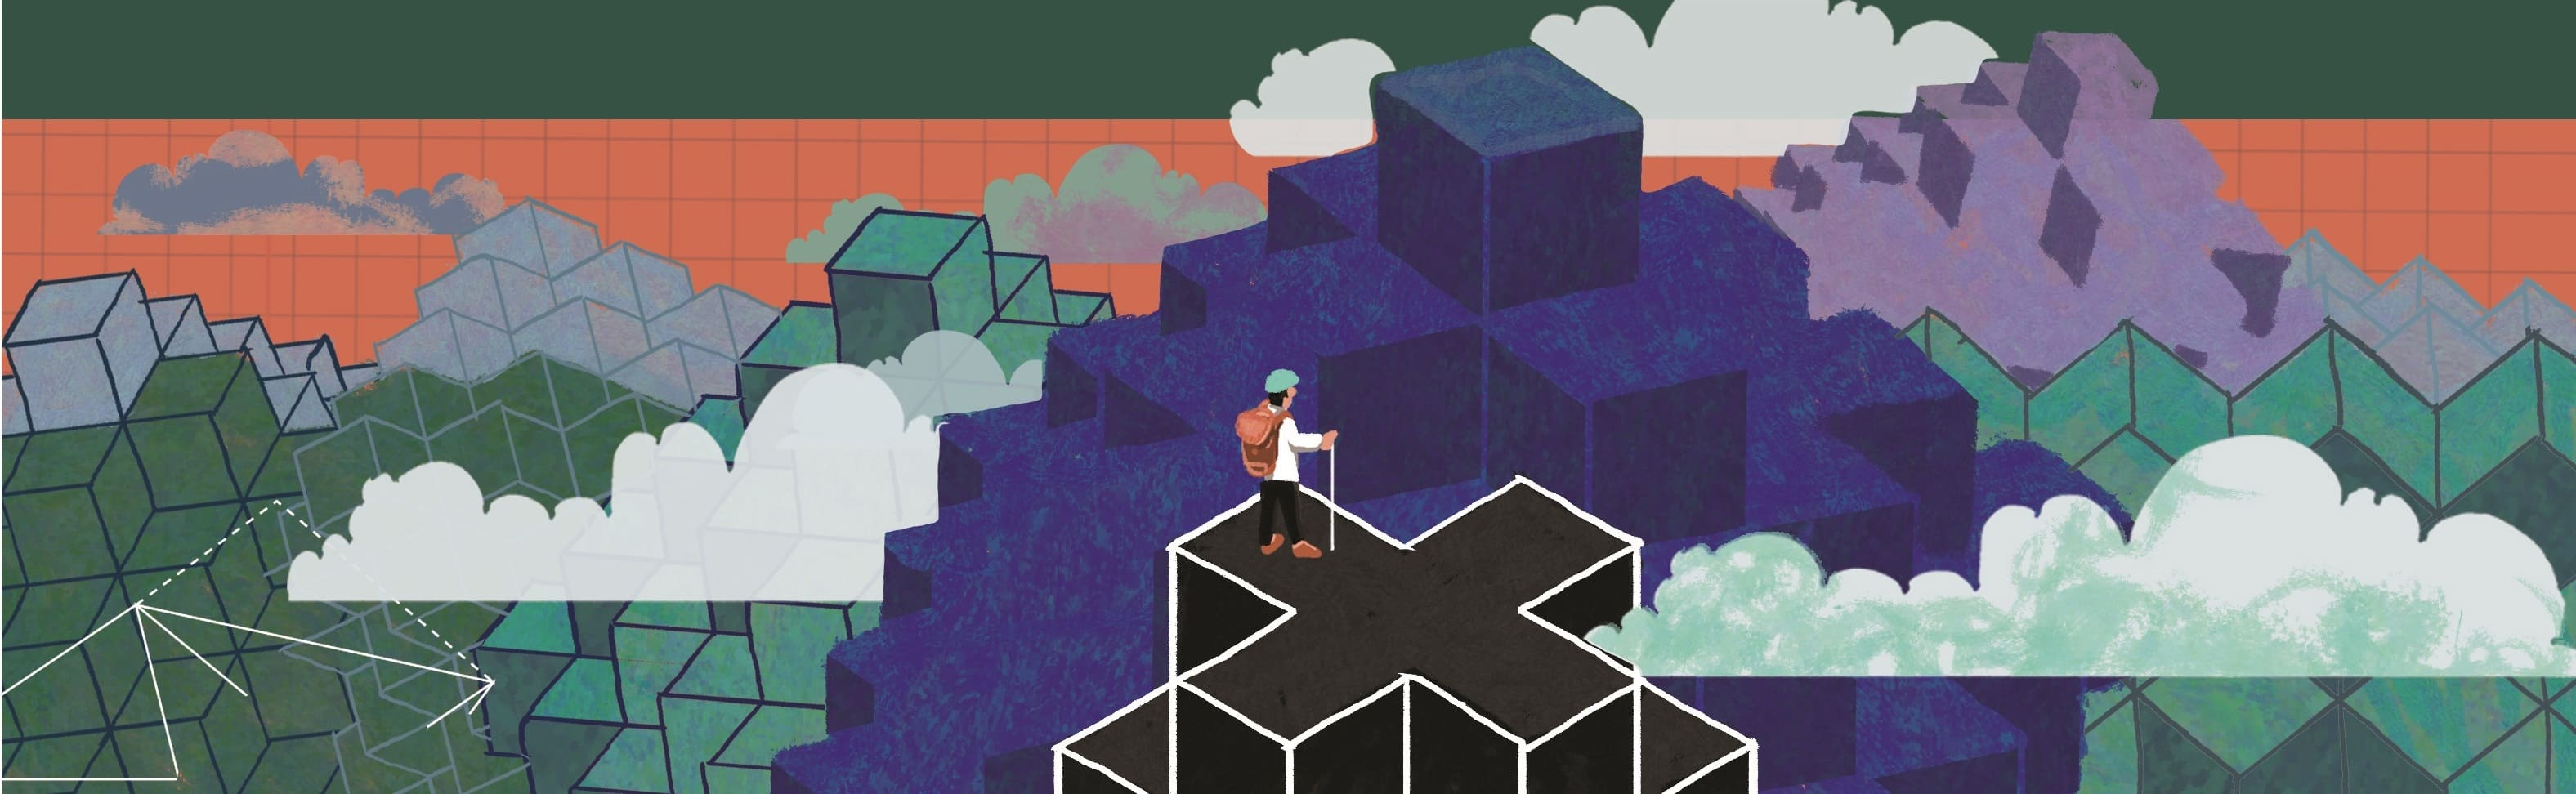
\includegraphics[width=19.3cm]{../thachthuctoanhoc/bannerthachthuc}}}
\centering
\vspace*{4cm}
\endgroup
\vspace*{-8pt}
\begin{tBox}
	\begin{itemize}[leftmargin = 13pt, itemsep = 1.0pt] 
		\item Mỗi bài toán đề xuất (kèm theo lời giải) cần được nêu rõ là bài sáng tác hay bài sưu tầm.
		%		\item Mỗi bài toán đề xuất (kèm theo lời giải) cần được nêu rõ là bài sáng tác hay bài sưu tầm (nếu là bài sưu tầm, cần ghi rõ nguồn).
		\item Bài giải cho mỗi bài toán cần được trình bày trong một file riêng hoặc
		một tờ giấy riêng.
		\item  Người đề xuất bài toán hoặc gửi bài giải cho các bài toán trong mục ``Thách thức kỳ này" cần ghi rõ họ, đệm, tên và nơi làm việc/học tập, số điện thoại liên hệ. Nếu là học sinh (hoặc sinh viên) cần ghi rõ là học sinh lớp mấy (hoặc sinh viên năm thứ mấy).
		\item Các bài toán trong mục Thách thức kỳ này hướng tới các độc giả là học sinh phổ thông; được phân chia thành các mức độ $B$, $A$, và được sắp xếp theo độ khó tăng dần, theo đánh giá chủ quan của Ban biên tập. Các bài toán mức độ $B$ không đòi hỏi các kiến thức vượt quá chương trình môn Toán cấp THCS; các bài toán mức độ $A$ không đòi hỏi các kiến thức vượt quá chương trình môn Toán cấp THPT.
		\item Cách thức gửi bài toán đề xuất hoặc lời giải: gửi file thu được bằng cách scan, ảnh chụp (rõ nét) của bản viết tay, hoặc được soạn thảo bằng các phần mềm Latex, Word tới \url{bbt@pi.edu.vn} hoặc gửi qua đường bưu điện tới Tòa soạn (xem địa chỉ tại bìa $2$).
		\item Hạn gửi lời giải cho các bài toán P$751$--P$760$: trước ngày $15/12/2023$.
	\end{itemize}
\end{tBox}
\begin{center}
	\vspace*{-5pt}
	\textbf{\color{thachthuctoanhoc}\color{thachthuctoanhoc}\color{thachthuctoanhoc}\color{thachthuctoanhoc}\color{thachthuctoanhoc}THÁCH THỨC KỲ NÀY}
	\vspace*{-5pt}
\end{center}
\begin{multicols}{2}
	\setlength{\abovedisplayskip}{4pt}
	\setlength{\belowdisplayskip}{4pt}
	{\color{thachthuctoanhoc}{\usefont{T5}{qag}{b}{n} P751.}}
	(Mức $B$) Người ta ghép khít năm hình chữ nhật bằng nhau với nhau, để được một hình dài $27$cm và rộng $15 $cm, như ở hình vẽ dưới đây. Biết rằng, đoạn thẳng $A C$ chia hình đó thành hai phần có diện tích bằng nhau. Hãy tính độ dài đoạn thẳng $A B$.
	\begin{figure}[H]
		\vspace*{-10pt}
		\centering
		\captionsetup{labelformat= empty, justification=centering}
		\definecolor{qqqqff}{rgb}{0,0,1}
		\begin{tikzpicture}[scale=0.5,thachthuctoanhoc, node font=\small]
			\draw  (-4,2)-- (-4,-2);
			\draw  (-4,-2)-- (-0.42,-2);
			\draw  (-0.42,-2)-- (-0.42,4);
			\draw  (-4,2)-- (6.74,2);
			\draw  (6.74,2)-- (6.74,4);
			\draw  (6.74,4)-- (-0.42,4);
			\draw  (3.16,4)-- (3.16,0);
			\draw  (3.16,0)-- (-4,0);
			\draw  (-4,-2)-- (4.5,4);
			\draw[decoration={brace,mirror,raise=5pt},decorate]
			(-4,-3) -- node[below = 6pt] {$27\text{ cm}$} (6.74,-3);
			\draw[decoration={brace,mirror,raise=5pt},decorate]
			(-4.5,4) -- node[left = 5pt] {$15\text{ cm}$} (-4.5,-2);
			\draw [fill=white] (-4,-2) circle (1.5pt);
			\draw (-4.08,-2.52) node {$C$};
			\draw [fill=white] (6.74,4) circle (1.5pt);
			\draw (6.74,4.5) node {$B$};
			\draw [fill=white] (4.5,4) circle (1.5pt);
			\draw (4.5,4.5) node {$A$};
		\end{tikzpicture}
		\vspace*{-10pt}
	\end{figure}
	\begin{flushright}
		\textit{Đăng Hải, Hà Nội (st)}
	\end{flushright}
	{\color{thachthuctoanhoc}{\usefont{T5}{qag}{b}{n} P752.}}
	(Mức $B$) Cho $x,y,z$ là các số thực thoả mãn $x^2y+y^2z+z^2x=1$ và $xy^2+yz^2+zx^2=2$. Tính giá trị biểu thức
	\begin{align*}
		P=\left(\!x^2\!+\!xy\!+\!y^2\!\right)\!\left(\!y^2\!+\!yz\!+\!z^2\!\right)\!\left(\!z^2\!+\!zx\!+\!x^2\!\right).
	\end{align*}
	\begin{flushright}
		\textit{Trần Quốc Luật, Tp. Hồ Chí Minh}
	\end{flushright}
	{\color{thachthuctoanhoc}{\usefont{T5}{qag}{b}{n} P753.}}
	(Mức $B$) Cho đường tròn $(O)$ với đường kính $AB = 2R$. Gọi $C$ là trung điểm của $OA$. $M$ là một điểm nằm trên $(O)$. Đường thẳng $MC$ cắt $(O)$ tại điểm thứ hai $D$.  Đường thẳng qua $D$ và vuông góc với $AB$, cắt $(O)$ tại điểm thứ hai $E$. Đường thẳng $ME$ cắt đường thẳng $AB$ tại điểm $F$. Tìm vị trí của điểm $M$  sao cho tổng $EF + MC$ có giá trị nhỏ nhất.
	\begin{figure}[H]
%		\vspace*{5pt}
		\centering
		\captionsetup{labelformat= empty, justification=centering}
		\definecolor{qqwuqq}{rgb}{0.,0.39215686274509803,0.}
		\definecolor{uuuuuu}{rgb}{0.26666666666666666,0.26666666666666666,0.26666666666666666}
		\definecolor{xdxdff}{rgb}{0.49019607843137253,0.49019607843137253,1.}
		\definecolor{ududff}{rgb}{0.30196078431372547,0.30196078431372547,1.}
		\begin{tikzpicture}[thachthuctoanhoc]
			\draw[color=qqwuqq,fill=qqwuqq,fill opacity=0.10000000149011612] (-1.5617418181909823,1.) -- (-1.5617418181909823,1.1880461622337974) -- (-1.7497879804247796,1.1880461622337974) -- (-1.7497879804247796,1.) -- cycle; 
			\draw  (0.,1.) circle (2.cm);
			\draw  (-2.,1.)-- (2.,1.);
			\draw  (-4.,1.)-- (0.4991521613769648,2.936710386142622);
			\draw  (0.4991521613769648,2.936710386142622)-- (-1.7497879804247796,0.03137105991975908);
			\draw  (-2.,1.)-- (-4.,1.);
			\draw  (-1.7497879804247796,1.968628940080241)-- (-1.7497879804247796,0.03137105991975908);
				\draw [fill=white] (0.,1.) circle (1.5pt);
				\draw (0.09082211690268885,1.2491318135923188) node {$O$};
				\draw [fill=white] (-2.,1.) circle (1.5pt);
				\draw (-2.2228335500515635,0.7335225357666101) node {$A$};
				\draw [fill=white] (2.,1.) circle (1.5pt);
				\draw (2.2449153240669926,0.9831943806090713) node {$B$};
				\draw [fill=white] (-1.,1.) circle (1.5pt);
				\draw (-1.0793025882235996,1.2757255568906436) node {$C$};
				\draw [fill=white] (0.4991521613769648,2.936710386142622) circle (1.5pt);
				\draw (0.6492907261675084,3.2170688176683497) node {$M$};
				\draw [fill=white] (-1.7497879804247796,0.03137105991975908) circle (1.5pt);
				\draw (-1.9435992454191537,-0.1869303245172173) node {$D$};
				\draw [fill=white] (-1.7497879804247796,1.968628940080241) circle (1.5pt);
				\draw (-1.917005502120829,2.233100315630334) node {$E$};
				\draw [fill=white] (-4.,1.) circle (1.5pt);
				\draw (-4.00461435103932,0.737413058716358) node {$F$};
		\end{tikzpicture}
		\vspace*{-10pt}
	\end{figure}
	\begin{flushright}
		\textit{Trần Thanh Hưng, Phú Yên}
	\end{flushright}
	{\color{thachthuctoanhoc}{\usefont{T5}{qag}{b}{n} P754.}}
	(Mức $B$) Cho $a, b, c$ là các số thực dương. Chứng minh rằng
	\begin{align*}
		&\frac{b+c}{\sqrt{\!a^2\!+\!b c}\!+\!\!\sqrt{\!a(b+c)}}\!+\!\frac{c\!+\!a}{\sqrt{\!b^2\!+\!c a}\!+\!\!\sqrt{\!b(c\!+\!a)}}\\
		&+\frac{a+b}{\sqrt{c^2+a b}+\sqrt{c(a+b)}} \geq \frac{3}{\sqrt{2}} .
	\end{align*}
	\begin{flushright}
		\textit{Nguyễn Việt Hùng, Hà Nội}
	\end{flushright}
	{\color{thachthuctoanhoc}{\usefont{T5}{qag}{b}{n} P755.}}
	(Mức $B$) Trong một hình chữ nhật có kích thước $5\times 10$, lấy $1351$ điểm đôi một phân biệt tuỳ ý. Chứng minh rằng, tồn tại một hình tròn bán kính bằng $\dfrac14$ chứa ít nhất $4$ điểm trong số các điểm đã lấy.
	\begin{flushright}
		\textit{Phạm Nhật Nguyệt, Hải Phòng (st)}
	\end{flushright}
	{\color{thachthuctoanhoc}{\usefont{T5}{qag}{b}{n} P756.}}
	(Mức $B$) Ta gọi số nguyên dương $n$ là ``số đẹp" nếu trong $22$ số: $5,n+5,2n+5,\ldots,21n+5$, tồn tại một số có cùng số dư với tích tất cả các số đó, trong phép chia cho $23$. Hãy tìm tất cả các số đẹp.
	\begin{flushright}
		\textit{Hà Duy Hưng, Hà Nội}
	\end{flushright}
	{\color{thachthuctoanhoc}{\usefont{T5}{qag}{b}{n} P757.}}
	(Mức $A$) Với mỗi số nguyên dương $n$, ta kí hiệu $a_n$ là nghiệm thực lớn nhất của phương trình
	\begin{align*}
		x^{2023}-nx^{2022}-nx^{2021}-\cdots-nx+1=0
	\end{align*}
	Xác định tất cả các số thực $C$, để 
	\begin{align*}
		a_1+\cdots+a_n>C. n^2
	\end{align*}
	với mọi số nguyên dương $n$.
	\begin{flushright}
		\textit{Tô Trung Hiếu, Nghệ An}
	\end{flushright}
	{\color{thachthuctoanhoc}{\usefont{T5}{qag}{b}{n} P758.}}
	(Mức $A$) Tìm số thực $k$ lớn nhất sao cho: 
	\begin{align*}
		a+b+c-3\ge k(a-b)(b-c)(c-a)
	\end{align*}
	với mọi số thực không âm $a,b,c$ thoả mãn $ab+bc+ca=3$. 
	\begin{flushright}
		\textit{Đinh Bình Dương, Hà Nội}
	\end{flushright}
	{\color{thachthuctoanhoc}{\usefont{T5}{qag}{b}{n} P759.}}
	(Mức $A$) Cho tam giác  $ABC$ nội tiếp đường tròn $(O)$, có các đường cao $BE,CF$ cắt nhau tại $H$.  Gọi $M, N$ tương ứng là trung điểm của $AH, EF$. Gọi $P$ là điểm đối xứng với $N$ qua $BC$. Chứng minh rằng $\angle BMP =\angle NMC$. 
	\begin{figure}[H]
		\vspace*{-5pt}
		\centering
		\captionsetup{labelformat= empty, justification=centering}
		\definecolor{qqwuqq}{rgb}{0,0.39215686274509803,0}
		\definecolor{ffqqqq}{rgb}{1,0,0}
		\definecolor{qqzzcc}{rgb}{0,0.6,0.8}
		\definecolor{qqqqff}{rgb}{0,0,1}
		\definecolor{qqqqffa}{rgb}{1,1,1}
		\begin{tikzpicture}[thachthuctoanhoc,scale=0.9]
			\draw [shift={(-2.4,1.2974770642201836)},color=qqwuqq] (0,0) -- (-115.88356340862376:0.6) arc (-115.88356340862376:-85.3246079752399:0.6) -- cycle;
			\draw [shift={(-2.4,1.2974770642201836)},color=qqwuqq] (0,0) -- (-70.77370689221246:0.6) arc (-70.77370689221246:-40.2147514588286:0.6) -- cycle;
			\draw (-0.592637676575393,0.4382959745607279) -- (-0.4280391340195052,0.20828006252750003) -- (-0.19802322198627734,0.37287860508338777) -- (-0.3626217645421651,0.6028945171166157) -- cycle; 
			\draw (-3.6432538877850886,-0.7848335552679585) -- (-3.3718647339119383,-0.8645074353041129) -- (-3.292190853875784,-0.5931182814309623) -- (-3.5635800077489344,-0.5134444013948081) -- cycle; 
			\draw [color=qqzzcc] (-2.4,3.45)-- (-4,-2);
			\draw [color=qqzzcc] (-4,-2)-- (1.5,-2);
			\draw [color=qqzzcc] (1.5,-2)-- (-2.4,3.45);
			\draw [color=ffqqqq] (-1.25,0.15252293577981646) circle (3.492256432316814cm);
			\draw  (-2.4,3.45)-- (-2.4,-0.855045871559633);
			\draw  (-3.5635800077489344,-0.5134444013948081)-- (-0.3626217645421651,0.6028945171166157);
			\draw  (-4,-2)-- (-0.3626217645421651,0.6028945171166157);
			\draw  (-3.5635800077489344,-0.5134444013948081)-- (1.5,-2);
			\draw  (-1.9631008861455497,-4.044725057860903)-- (-1.9631008861455497,0.044725057860903805);
			\draw  (-1.9631008861455497,0.044725057860903805)-- (-2.4,1.2974770642201836);
			\draw  (-2.4,1.2974770642201836)-- (1.5,-2);
			\draw  (-4,-2)-- (-2.4,1.2974770642201836);
			\draw  (-2.4,1.2974770642201836)-- (-1.9631008861455497,-4.044725057860903);
			\draw [shift={(-2.4,1.2974770642201836)},color=qqwuqq] (-115.88356340862376:0.6) arc (-115.88356340862376:-85.3246079752399:0.6);
			\draw[color=qqwuqq] (-2.4993715787134962,0.766699060395621) -- (-2.5214541517609392,0.6487483928790517);
			\draw [shift={(-2.4,1.2974770642201836)},color=qqwuqq] (-70.77370689221246:0.6) arc (-70.77370689221246:-40.2147514588286:0.6);
			\draw[color=qqwuqq] (-2.094095810427579,0.8524797307427333) -- (-2.026117101633708,0.7535914344144113);
			\draw [fill=white] (-2.4,3.45) circle (1.5pt);
			\draw (-2.6,4.04) node {$A$};
			\draw [fill=white] (-4,-2) circle (1.5pt);
			\draw (-4.32,-2.26) node {$B$};
			\draw [fill=white] (1.5,-2) circle (1.5pt);
			\draw (1.7,-2.2) node {$C$};
			\draw [fill=white] (-0.3626217645421651,0.6028945171166157) circle (1.5pt);
			\draw (-0.2,0.92) node {$E$};
			\draw [fill=white] (-3.5635800077489344,-0.5134444013948081) circle (1.5pt);
			\draw (-3.94,-0.52) node {$F$};
			\draw [fill=white] (-2.4,-0.855045871559633) circle (1.5pt);
			\draw (-2.5,-1.22) node {$H$};
			\draw [fill=white] (-1.9631008861455497,0.044725057860903805) circle (1.5pt);
			\draw (-1.76,-0.15) node {$N$};
			\draw [fill=white] (-2.4,1.2974770642201836) circle (1.5pt);
			\draw (-2.18,1.68) node {$M$};
			\draw [fill=white] (-1.9631008861455497,-4.044725057860903) circle (1.5pt);
			\draw (-2,-4.36) node {$P$};
		\end{tikzpicture}
		\vspace*{-10pt}
	\end{figure} 
	\begin{flushright}
		\textit{Lưu Công Đông, Hà Nội}
	\end{flushright}
	{\color{thachthuctoanhoc}{\usefont{T5}{qag}{b}{n} P760.}}
	(Mức $A$) Cho dãy số $(x_n)$ xác định bởi $x_1=4$ và 
	\begin{align*}
			&x_{n+1}=45x_n+\sqrt{2024x_n^2+16}\\
			&\text{với mọi số nguyên dương $n$}.
	\end{align*}
	Tìm tất cả các số nguyên $a$ sao cho: $a^n\left(\dfrac{x_{2n}}{x_n}+2\right)$ là số chính phương với mọi số nguyên dương $n$.
	\begin{flushright}
		\textit{Nguyễn Đức Khải, Nam Định}
	\end{flushright}
\end{multicols}
\newpage
\centerline{{\large{\textbf{\color{thachthuctoanhoc}\color{thachthuctoanhoc}\color{thachthuctoanhoc}GIẢI BÀI KỲ TRƯỚC}}}}
\vspace*{-5pt}
\begin{multicols}{2}
	\setlength{\abovedisplayskip}{5pt}
	\setlength{\belowdisplayskip}{5pt}
	{\color{thachthuctoanhoc}{\usefont{T5}{qag}{b}{n} P720.}}
	(Mức $A$) Một thành phố có $1332$ căn nhà. Mỗi dịp Noel, Ông già Noel sẽ đến thăm các căn nhà đó theo thứ tự tùy ý. Chứng minh rằng, có thể tìm được $12$ căn nhà trong thành phố đó, sao cho trong ba năm liên tiếp, có ít nhất hai năm mà Ông già Noel đến thăm $12$ căn nhà đó theo cùng một thứ tự.
	\vskip 0.05cm
	\textbf{\color{thachthuctoanhoc}Lời giải} (\textit{dựa theo Đáp án của bài toán})\textbf{\color{thachthuctoanhoc}.}
	\vskip 0.05cm
	Trước hết, ta nhắc lại kết quả nổi tiếng sau:
	\vskip 0.05cm
	\textbf{\color{thachthuctoanhoc}Định lý Erdos -- Szekeres.} Cho các số nguyên dương $p, q > 1$. Khi đó, mỗi dãy $(p - 1)(q - 1) + 1$ số thực đôi một phân biệt sẽ chứa một dãy con tăng có $p$ số hạng, hoặc chứa một dãy con giảm có $q$ số hạng.
	\vskip 0.05cm
	\textit{Chứng minh.}
	\vskip 0.1cm
	Đặt $N = (p - 1)(q - 1) + 1$.
	\vskip 0.05cm
	Xét dãy số thực $x_1,x_2,\ldots,x_N$ tùy ý, thỏa mãn $x_i \ne x_j$, với mọi $i, j \in \{1; 2; \ldots; N\}$ và $i \ne j$.
	\vskip 0.05cm
	Với mỗi $i \in \{1; 2; \ldots; N\}$, ký hiệu $d_i$ là số các số hạng của dãy con tăng có nhiều số hạng nhất và có $x_i$ là số hạng có giá trị lớn nhất; ký hiệu $n_i$ là số các số hạng của dãy con giảm có nhiều số hạng nhất và có  $x_i$ là số hạng có giá trị bé nhất.
	\vskip 0.05cm
	Xét các cặp số $\left(d_i, n_i\right),  i = 1, 2, \ldots, N$.
	\vskip 0.05cm
	Dễ thấy, với $1 \le i < j \le N$, ta có  $d_i < d_j$ nếu  $x_i < x_j$, và $n_i < n_j$  nếu $x_i > x_j$.
	\vskip 0.05cm
	Vì vậy, $N$ cặp $\left(d_i, n_i\right), i = 1, 2, \ldots, N$, đôi một khác nhau.     \hfill ($1$)
	\vskip 0.05cm
	Nhận thấy, nếu với mọi $i \in \{1; 2; \ldots; N\}$, $1 \le d_i \le p-1$  và $1 \le n_i \le q-1$, thì trong $N$ cặp $\left(d_i, n_i\right), i = 1, 2, \ldots, N$, chỉ có tối đa $(p - 1)(q - 1)$ cặp đôi một khác nhau, mâu thuẫn với ($1$) (do $(p - 1)(q - 1) < N$). Vì vậy, phải tồn tại $i \in \{1; 2; \ldots; N\}$ sao cho $d_i \ge p$, hoặc tồn tại $j \in \{1; 2; \ldots; N\}$ sao cho $n_j \ge q$. Từ đây, hiển nhiên ta có điều phải chứng minh theo yêu cầu của định lý.
	\vskip 0.01cm
	\textit{Trở lại bài toán.}
	\vskip 0.01cm
	Xét ba năm liên tiếp tùy ý.
	\vskip 0.01cm
	Ở năm thứ nhất, theo chân Ông già Noel, ta lần lượt đánh số các căn nhà mà Ông tới thăm, bởi$ 1, 2, \ldots, 1332$. Ta sẽ gọi căn nhà được đánh số $i$ là căn nhà $i$.
	\vskip 0.01cm
	Khi đó, ở năm thứ hai, liệt kê các căn nhà theo thứ tự mà Ông già Noel lần lượt tới thăm, ta sẽ thu được một hoán vị của $1, 2, \ldots, 1332$:
	\begin{align*}
		{a_1},{a_2}, \ldots ,{a_{1332}}. \tag{$2$}
	\end{align*}
	Dễ thấy, nếu trong dãy ($2$) tồn tại một dãy con tăng có $12$ số hạng thì $12$ số hạng của dãy con đó sẽ là $12$ số hạng nằm theo cùng một thứ tự trong dãy $1, 2, \ldots, 1332$ và trong dãy ($2$). Vì thế, ta có $12$ căn nhà, mà Ông già Noel tới thăm ở năm thứ nhất và năm thứ hai theo cùng một thứ tự.
	\vskip 0.01cm
	Xét trường hợp ngược lại, trong dãy ($2$) không tồn tại một dãy con tăng có $12$ số hạng.
	\vskip 0.01cm
	Khi đó, do
	\begin{align*}
		1332 = (12 - 1)(122 - 1) + 1,
	\end{align*}
	nên theo định lý Erdos -- Szekeres, trong dãy ($2$) phải tồn tại một dãy con giảm có $122$ số hạng. Giả sử dãy con đó là
	\begin{align*}
		{a_{{i_1}}},{a_{{i_2}}}, \ldots ,{a_{{i_{122}}}}. \tag{$3$}
	\end{align*}
	Xét năm thứ ba. Giả sử trong năm này, Ông già Noel tới thăm các căn nhà thuộc dãy ($3$) theo thứ tự:
	\begin{align*}
		{a_{{j_1}}},{a_{{j_2}}}, \ldots ,{a_{{j_{122}}}}. \tag{$4$}
	\end{align*}
	Dễ thấy, nếu trong dãy ($4$) tồn tại một dãy con tăng có $12$ số hạng thì $12$ số hạng của dãy con đó sẽ là $12$ số hạng nằm trong dãy $1, 2, \ldots, 1332$ và dãy ($4$) theo cùng một thứ tự. Vì thế, ta có $12$ căn nhà, mà Ông già Noel tới thăm ở năm thứ nhất và năm thứ ba theo cùng một thứ tự.
	\vskip 0.05cm
	Xét trường hợp ngược lại, trong dãy ($4$) không tồn tại một dãy con tăng có $12$ số hạng.
	\vskip 0.05cm
	Khi đó, do
	\begin{align*}
		122 = (12 - 1)(12 - 1) + 1,
	\end{align*}
	nên theo định lý Erdos -- Szekeres, trong dãy ($4$) phải tồn tại một dãy con giảm có $12$ số hạng; ký hiệu dãy con này là ($5$).
	\vskip 0.05cm
	Do tất cả $12$ số hạng của dãy ($5$) đều là số hạng của dãy ($3$), và do cả hai dãy ($3$), ($5$) cùng là dãy giảm, nên tất cả $12$ số hạng của dãy ($5$) nằm trong dãy ($3$) và dãy ($4$) theo cùng một thứ tự. Vì thế, ta có $12$ căn nhà, mà Ông già Noel tới thăm ở năm thứ hai và năm thứ ba theo cùng một thứ tự.
	\vskip 0.05cm
	Kết quả xét các trường hợp có thể xảy ra trên đây cho ta điều phải chứng minh theo yêu cầu đề bài.
	\vskip 0.05cm
	\textbf{\color{thachthuctoanhoc}Bình luận và Nhận xét}
	\vskip 0.05cm
	Cho tới thời điểm bản thảo vào Nhà in, Tạp chí vẫn chưa nhận được lời giải nào từ bạn đọc.
	\vskip 0.05cm
	\hfill	\textbf{\color{thachthuctoanhoc}Nguyễn Khắc Minh}
	\vskip 0.05cm
	{\color{thachthuctoanhoc}{\usefont{T5}{qag}{b}{n} P721.}}
	(Mức $B$)
	Trên mỗi cạnh của một hình vuông, bạn An viết một số nguyên dương. Sau đó, tại mỗi đỉnh của hình vuông đó, bạn An viết một số bằng tích của hai số đã được viết ở hai cạnh đi qua đỉnh đó. Biết rằng, tổng các số ở các đỉnh của hình vuông bằng $1333$. Hỏi, tổng các số được viết ở các cạnh của hình vuông đó có thể bằng bao nhiêu?
	\vskip 0.05cm
	\textbf{\color{thachthuctoanhoc}Lời giải} (\textit{dựa theo ý giải của một bạn học sinh cấp THCS})\textbf{\color{thachthuctoanhoc}.}
	\vskip 0.05cm
	Giả sử các số nguyên dương được viết ở các cạnh của hình vuông, tính theo chiều kim đồng hồ, lần lượt là $a, b, c, d$.
	\vskip 0.05cm
	Khi đó, các số được viết ở bốn đỉnh của hình vuông đó sẽ là $ab$, $bc$, $cd$ và $da$.
	\vskip 0.05cm
	Theo giả thiết của bài ra, ta có:
	\begin{align*}
		31 \cdot 43 &= 1333 = ab + bc + cd + da \\
		&= \left( a + c \right)\left( b + d \right) . \tag{$*$}
	\end{align*}
	Do $a + c, b + d$ là các số nguyên dương lớn hơn $1$ (vì $a,b,c,d \in \mathbb{N^*}$) và $31$, $43$ là các số nguyên tố, nên
	\begin{align*}
		\left( *  \right) \Leftrightarrow \left( {a + c,b + d} \right) \in \left\{ {\left( {31,43} \right);\left( {43,31} \right)} \right\}.
	\end{align*}
	Vì vậy, $a + b + c + d = 31 + 43 = 74$.
	\vskip 0.05cm
	Vậy, tổng các số được viết ở các cạnh của hình vuông bằng $74$.
	\vskip 0.05cm
	\textbf{\color{thachthuctoanhoc}Bình luận và Nhận xét}
	\vskip 0.05cm	
	Tuy bài đã ra là một bài toán đơn giản, nhưng rất tiếc, trong số các lời giải Tạp chí đã nhận được từ bạn đọc, có một số lời giải thiếu chặt chẽ, thiếu chính xác, do người giải bài đã mắc một trong các lỗi chuyên môn sau:
	\vskip 0.05cm
	-- Bỏ sót phân tích $1333 = 1 \cdot 1333$, khi xét các phân tích số $1333$ thành tích của hai số nguyên dương;
	\vskip 0.05cm
	-- Thiếu khẳng định $1333$ chỉ có đúng hai cách phân tích thành tích của hai số nguyên dương, là
	\begin{align*}
		1333 = 1 \cdot 1333 \text{ và } 1333 = 31 \cdot 43.
	\end{align*}  
	\begin{flushright}
		\textbf{\color{thachthuctoanhoc}Hà Thanh}
	\end{flushright}
	{\color{thachthuctoanhoc}{\usefont{T5}{qag}{b}{n} P722.}}
	(Mức $B$)
	Cho $a, b, c$ là các số thực khác $0$, thỏa mãn:
	\begin{align*}
		\begin{cases}
			a + b + c = \dfrac{1}{a} + \dfrac{1}{b} + \dfrac{1}{c}\\
			{a^3} + {b^3} + {c^3} = \dfrac{1}{{{a^3}}} + \dfrac{1}{{{b^3}}} + \dfrac{1}{{{c^3}}}.
		\end{cases}
	\end{align*}
	Chứng minh rằng
	\begin{align*}
		{a^{2023}} \!+\! {b^{2023}} \!+\! {c^{2023}} \!=\! \frac{1}{{{a^{2023}}}} \!+\! \frac{1}{{{b^{2023}}}} \!+\! \frac{1}{{{c^{2023}}}}.
	\end{align*}
	\textbf{\color{thachthuctoanhoc}Lời giải} (\textit{của người chấm bài})\textbf{\color{thachthuctoanhoc}.}
	\vskip 0.05cm
	Đặt $x = a - \dfrac{1}{a}$, $y = b - \dfrac{1}{b}$  và $z = c - \dfrac{1}{c}$.
	\vskip 0.05cm
	Theo giả thiết của bài ra, ta có:
	\begin{align*}
		\hspace*{-5pt}x \!+\! y \!+\! z \!=\! \left( {a \!+\! b \!+\! c} \right) \!-\! \left(\!\! {\frac{1}{a} \!+\! \frac{1}{b} \!+\! \frac{1}{c}} \!\!\right) \!=\! 0, \tag{$1$}
	\end{align*}
	và
	\begin{align*}
		&{x^3} + {y^3} + {z^3} \\
		= \,&{\left( {a - \frac{1}{a}} \right)^3} + {\left( {b - \frac{1}{b}} \right)^3} + {\left( {c - \frac{1}{c}} \right)^3}\\
		= \,&\left( {{a^3} + {b^3} + {c^3} - \frac{1}{{{a^3}}} - \frac{1}{{{b^3}}} - \frac{1}{{{c^3}}}} \right) \\
		&- 3\left( {a + b + c - \frac{1}{a} - \frac{1}{b} - \frac{1}{c}} \right)\\
		 = \,\,& 0.\tag{$2$}
	\end{align*}
	Từ ($1$) suy ra $x + y = -z$. Do đó, từ ($2$) ta được:
	\begin{align*}
		0 &= {x^3} \!+\! {y^3} \!+\! {z^3} = {\left( {x \!+\! y} \right)^3} \!-\! 3xy\left( {x \!+\! y} \right) \!+\! {z^3} \\
		&= {\left( { - z} \right)^3} + 3xyz + {z^3} = 3xyz.
	\end{align*}
	Vì vậy, $x = 0$, hoặc $y = 0$, hoặc $z = 0$. Điều này cho thấy, trong ba số $a, b, c$, có ít nhất một số bằng nghịch đảo của nó.
	\vskip 0.05cm
	Do vai trò của $a, b, c$ trong bài toán hoàn toàn như nhau, nên không mất tính tổng quát, giả sử
	\begin{align*}
		a = \frac{1}{a}. \tag{$3$}
	\end{align*}
	Khi đó, từ giả thiết
	\begin{align*}
		a + b + c = \frac{1}{a} + \frac{1}{b} + \frac{1}{c},
	\end{align*}
	suy ra
	\begin{align*}
		b + c = \frac{1}{b} + \frac{1}{c} = \frac{{b + c}}{{bc}}.
	\end{align*}
	Do đó, $b + c = 0$ hoặc $bc = 1$.
	\vskip 0.05cm
	-- Nếu $b + c = 0$ thì $b = - c$. Từ đây và ($3$), suy ra
	\begin{align*}
		&{a^{2023}} + {b^{2023}} + {c^{2023}}\\
		 = \,&\frac{1}{{{a^{2023}}}} + {\left( { - c} \right)^{2023}} + {c^{2023}}\\
		  = \,&\frac{1}{{{a^{2023}}}} = \frac{1}{{{a^{2023}}}} + \frac{1}{{{{\left( { - c} \right)}^{2023}}}} + \frac{1}{{{c^{2023}}}}\\
		   = \,&\frac{1}{{{a^{2023}}}} + \frac{1}{{{b^{2023}}}} + \frac{1}{{{c^{2023}}}}.
	\end{align*}
	-- Nếu $bc = 1$ thì
	\begin{align*}
			&\frac{1}{{{a^{2023}}}} + \frac{1}{{{b^{2023}}}} + \frac{1}{{{c^{2023}}}} \\
			= \,\,&{a^{2023}} + \frac{{{b^{2023}} + {c^{2023}}}}{{{{\left( {bc} \right)}^{2023}}}} \quad({\text {do }} (3))\\
			 = \,\,&{a^{2023}} + {b^{2023}} + {c^{2023}}.
	\end{align*}
	Vì vậy, ta có điều phải chứng minh theo yêu cầu đề bài.
	\vskip 0.05cm
	\textbf{\color{thachthuctoanhoc}Bình luận và Nhận xét}
	\vskip 0.05cm
	$\pmb{1.}$ Ở bài đã ra, nếu thay giả thiết
	\begin{align*}
		{a^3} + {b^3} + {c^3} = \frac{1}{{{a^3}}} + \frac{1}{{{b^3}}} + \frac{1}{{{c^3}}},
	\end{align*}
	bởi giả thiết ``$|abc| = 1$", ta có thể dễ dàng chứng minh được rằng
	\begin{align*}
		{a^n} + {b^n} + {c^n} = \frac{1}{{{a^n}}} + \frac{1}{{{b^n}}} + \frac{1}{{{c^n}}},
	\end{align*}
	với mọi số nguyên dương $n > 1$.
	\vskip 0.05cm
	$\pmb{2.}$ Trong số các lời giải Tạp chí đã nhận được từ bạn đọc, rất tiếc, có ba lời giải sai, do người giải bài đã mắc ít nhất một trong các lỗi chuyên môn sau:
	\vskip 0.05cm
	-- Chưa xét hết các trường hợp có thể xảy ra đối với $a, b, c$;
	\vskip 0.05cm
	-- Nhầm lẫn giữa ``hoặc" và ``đồng thời".
	\begin{flushright}
		\textbf{\color{thachthuctoanhoc}Hà Thanh}
	\end{flushright}
	{\color{thachthuctoanhoc}{\usefont{T5}{qag}{b}{n} P723.}}
	(Mức $B$) Cho số nguyên dương $k$ và cho $A$ là số tự nhiên gồm $k$ chữ số $9$. Gọi $m, n, p$ tương ứng là tổng các chữ số của $A$, $A^2$, $A^3$. Chứng minh rằng $p = 2m = 2n$.
	\vskip 0.05cm
	\textbf{\color{thachthuctoanhoc}Lời giải} (\textit{dựa theo lời giải của bạn Nguyễn Chánh Thiện, lớp $9/12$, trường THCS Lê Quý Đôn, Quận 3, Tp. Hồ Chí Minh})\textbf{\color{thachthuctoanhoc}.}
	\vskip 0.05cm
	Theo giả thiết của bài ra, $A = \underbrace {99 \ldots 9}_{k{\text{ c/s }}9}.$ \hfill ($1$)
	\vskip 0.05cm
	Vì vậy, $m = 9k$. \hfill ($2$)
	\vskip 0.05cm
	Từ ($1$), ta có:
	\begin{align*}
			&{A^2} \\
			=& {\left( {{{10}^k} - 1} \right)^2} = {10^{2k}} - 2 \cdot {10^k} + 1 \\
			= &1\underbrace {0 \ldots 0}_{2k{\text{ c/s }}0} - 2\underbrace {0 \ldots 0}_{k {\text{ c/s }} 0} + 1 = \underbrace {9 \ldots 9}_{k - 1{\text{ c/s }}9}8\underbrace {0 \ldots 0}_{k - 1{\text{ c/s }}0}1.\\
				&{A^3} \\
				=& {\left( {{{10}^k} - 1} \right)^3} = {10^{3k}} - 3 \cdot {10^{2k}} + 3 \cdot {10^k} - 1\\
				 =& {10^{2k + 1}}\left( {{{10}^{k - 1}} - 1} \right) + 7 \cdot {10^{2k}} + 2 \cdot {10^k} \\
				 &+ {10^k} - 1\\
				 =& \underbrace {9 \ldots 9}_{k - 1{\text{ c/s }}9} \cdot {10^{2k + 1}} + 7 \cdot {10^{2k}} + 2 \cdot {10^k} + {10^k} - 1\\
				 =& \underbrace {9 \ldots 9}_{k - 1{\text{ c/s }}9}\underbrace {0 \ldots 0}_{2k + 1{\text{ c/s }}0} + 7\underbrace {0 \ldots 0}_{2k{\text{ c/s }}0} + 2\underbrace {0 \ldots 0}_{k{\text{ c/s }}0} + \underbrace {9 \ldots 9}_{k{\text{ c/s }}9}\\
				 =&\underbrace {9 \ldots 9}_{k - 1{\text{ c/s }}9}7\underbrace {0 \ldots 0}_{k - 1{\text{ c/s }}0}2\underbrace {9 \ldots 9}_{k{\text{ c/s }}9}.
	\end{align*}
	Vì vậy
	\begin{align*}
		&n = 9(k - 1) + 8 + 1 = 9k, \tag{$3$}\\
		&p = 9(k - 1) + 7 + 2 + 9k = 18k. \tag{$4$}
	\end{align*}
	Từ ($2$), ($3$) và ($4$), suy ra $p = 2m = 2n$, là điều phải chứng minh theo yêu cầu đề bài.
	\vskip 0.05cm
	\textbf{\color{thachthuctoanhoc}Bình luận và Nhận xét}
	\vskip 0.05cm
	Tất cả lời giải Tạp chí nhận được từ bạn đọc đều là lời giải đúng và hoàn chỉnh.
	\begin{flushright}
		\textbf{\color{thachthuctoanhoc}Lưu Thị Thanh Hà}
	\end{flushright}
	{\color{thachthuctoanhoc}{\usefont{T5}{qag}{b}{n} P724.}}
	(Mức $B$) Cho tam giác $ABC$. Trên các cạnh $BC, CA, AB,$ tương ứng, lấy các điểm $D, E, F,$ sao cho $AEDF$ là hình bình hành ($D, E, F$ không trùng với các đỉnh của tam giác). Gọi $Y$ là điểm đối xứng với $B$ qua $DF$; $Z$ là điểm đối xứng với $C$ qua $DE$. Chứng minh rằng, đường tròn ngoại tiếp tam giác $AYZ$ đi qua trực tâm của tam giác $ABC$.
	\vskip 0.05cm
	\textbf{\color{thachthuctoanhoc}Lời giải} (\textit{dựa theo Đáp án của BBT Tạp chí})\textbf{\color{thachthuctoanhoc}.}
	\vskip 0.05cm
	Gọi $H$ là trực tâm của tam giác $ABC$.
	\vskip 0.05cm
	Xét hai trường hợp sau:
	\vskip 0.05cm
	$\bullet$ \textit{Trường hợp $1$: $D$ không là trung điểm của $BC$.}
	\begin{figure}[H]
		\vspace*{-5pt}
		\centering
		\captionsetup{labelformat= empty, justification=centering}
		\definecolor{qqwuqq}{rgb}{0.,0.39215686274509803,0.}
		\definecolor{ffqqqq}{rgb}{1.,0.,0.}
		\definecolor{xdxdff}{rgb}{0.49019607843137253,0.49019607843137253,1.}
		\definecolor{uuuuuu}{rgb}{0.26666666666666666,0.26666666666666666,0.26666666666666666}
		\definecolor{qqqqff}{rgb}{0.,0.,1.}
		\definecolor{cqcqcq}{rgb}{0.7529411764705882,0.7529411764705882,0.7529411764705882}
		\begin{tikzpicture}[thachthuctoanhoc,scale=0.55]
			\draw[pattern color=qqwuqq,fill=qqwuqq,fill opacity=0.10000000149011612] (4.695618299023638,-2.) -- (4.695618299023638,-1.717157287525381) -- (4.412775586549019,-1.717157287525381) -- (4.412775586549019,-2.) -- cycle; 
			\draw[pattern color=qqwuqq,fill=qqwuqq,fill opacity=0.10000000149011612] (4.696510283066152,2.102774089908528) -- (4.8618107563320745,1.873262099942727) -- (5.091322746297876,2.03856257320865) -- (4.926022273031952,2.268074563174451) -- cycle; 
			\draw[pattern color=ffqqqq,fill=ffqqqq,fill opacity=0.10000000149011612] (5.8985388288815495,2.9685061483166395) -- (6.063839302147472,2.7389941583508386) -- (6.2933512921132735,2.9042946316167617) -- (6.12805081884735,3.1338066215825626) -- cycle; 
			\draw[pattern color=qqwuqq,fill=qqwuqq,fill opacity=0.10000000149011612] (0.31818451331543657,1.031668750812834) -- (0.5775689785900543,0.9188871070306979) -- (0.6903506223721905,1.1782715723053157) -- (0.43096615709757274,1.2910532160874517) -- cycle; 
			\draw[pattern color=ffqqqq,fill=ffqqqq,fill opacity=0.10000000149011612] (1.7068770930595383,0.7362808532744197) -- (1.5940954492774022,0.47689638799980205) -- (1.8534799145520198,0.3641147442176659) -- (1.966261558334156,0.6234992094922835) -- cycle; 
			\draw [shift={(0.8255511730980358,-2.)},pattern color=qqwuqq,fill=qqwuqq,fill opacity=0.10000000149011612] (0,0) -- (0.:0.4) arc (0.:54.23759050782091:0.4) -- cycle;
			\draw [shift={(9.825551173098036,-2.)},pattern color=qqwuqq,fill=qqwuqq,fill opacity=0.10000000149011612] (0,0) -- (125.7624094921791:0.4) arc (125.7624094921791:180.:0.4) -- cycle;
			\draw [shift={(8.,-2.)},pattern color=qqwuqq,fill=qqwuqq,fill opacity=0.10000000149011612] (0,0) -- (125.76240949217907:0.4) arc (125.76240949217907:180.:0.4) -- cycle;
			\draw[pattern color=ffqqqq,fill=ffqqqq,fill opacity=0.10000000149011612] (2.388,5.5091572875253805) -- (2.670842712474619,5.5091572875253805) -- (2.670842712474619,5.792) -- (2.388,5.792) -- cycle; 
			\draw  (2.388,5.792)-- (-1.,-2.);
			\draw  (-1.,-2.)-- (8.,-2.);
			\draw  (8.,-2.)-- (2.388,5.792);
			\draw  (5.7631662879681205,1.1057391810677832)-- (4.412775586549018,-2.);
			\draw  (4.412775586549018,-2.)-- (1.0376092985808971,2.6862608189322166);
			\draw (1.9,6.8) node[anchor=north west] {$A$};
			\draw (-1.5,-1.88) node[anchor=north west] {$B$};
			\draw (8.,-1.86) node[anchor=north west] {$C$};
			\draw (3.56,-1.89) node[anchor=north west] {$D$};
			\draw (5.76,1.66) node[anchor=north west] {$E$};
			\draw (0.48,3.5) node[anchor=north west] {$F$};
			\draw (6.12,3.72) node[anchor=north west] {$Y$};
			\draw (1.6,1.48) node[anchor=north west] {$Z$};
			\draw [color=ffqqqq] (3.300775586549017,3.116062628336754) circle (2.8273309124444386cm);
			\draw  (6.12805081884735,3.1338066215825626)-- (-1.,-2.);
			\draw  (0.43096615709757274,1.2910532160874517)-- (8.,-2.);
			\draw (2.02,0.44) node[anchor=north west] {$H$};
			\draw (0.82,-1.86) node[anchor=north west] {$C'$};
			\draw (9.82,-1.86) node[anchor=north west] {$B'$};
			\draw (6.44,6.44) node[anchor=north west] {$A'$};
			\draw  (2.388,5.792)-- (6.437551173098037,5.792);
			\draw  (6.437551173098037,5.792)-- (9.825551173098036,-2.);
			\draw  (9.825551173098036,-2.)-- (8.,-2.);
			\draw  (4.213551173098033,5.792)-- (0.8255511730980358,-2.);
			\draw (3.56,6.7) node[anchor=north west] {$K$};
			\draw [dash pattern=on 5pt off 5pt,color=qqqqff] (4.213551173098033,5.792)-- (9.825551173098036,-2.);
			\draw  (2.388,5.792)-- (0.8255511730980358,-2.);
			\draw  (8.,-2.)-- (6.437551173098037,5.792);
			\draw  (4.412775586549018,-2.62336)-- (4.412775586549018,6.640462222222222);
			\draw  (0.8255511730980358,-2.)-- (6.437551173098037,5.792);
			\draw (4.42,6.84) node[anchor=north west] {$d$};
			\draw  (2.388,0.4401252566735113)-- (2.388,5.792);
			\begin{scriptsize}
				\draw [fill=white] (2.388,5.792) circle (1.5pt);
				\draw [fill=white] (-1.,-2.) circle (1.5pt);
				\draw [fill=white] (8.,-2.) circle (1.5pt);
				\draw [fill=white] (1.0376092985808971,2.6862608189322166) circle (1.5pt);
				\draw [fill=white] (4.412775586549018,-2.) circle (1.5pt);
				\draw [fill=white] (5.7631662879681205,1.1057391810677832) circle (1.5pt);
				\draw [fill=white] (6.12805081884735,3.1338066215825626) circle (1.5pt);
				\draw [fill=white] (1.966261558334156,0.6234992094922835) circle (1.5pt);
				\draw [fill=ffqqqq] (2.388,0.4401252566735113) circle (1.5pt);
				\draw [fill=white] (4.926022273031952,2.268074563174451) circle (1.5pt);
				\draw [fill=white] (0.43096615709757274,1.2910532160874517) circle (1.5pt);
				\draw [fill=white] (0.8255511730980358,-2.) circle (1.5pt);
				\draw [fill=white] (9.825551173098036,-2.) circle (1.5pt);
				\draw [fill=white] (6.437551173098037,5.792) circle (1.5pt);
				\draw [fill=white] (4.213551173098033,5.792) circle (1.5pt);
			\end{scriptsize}
		\end{tikzpicture}
		\vspace*{-10pt}
	\end{figure}
	Gọi $d$ là đường thẳng vuông góc với $BC$ tại $D$. Gọi $A',B', C'$  tương ứng là điểm đối xứng với $A, B, C$ qua $d$. Gọi $K$ là giao điểm của  $C'Z$ và $AA'$.
	\vskip 0.05cm  
	Do $Z$ đối xứng với $C$ qua $DE$ (giả thiết) nên $DE$ là đường trung trực của $CZ$. Từ đây và định nghĩa điểm $C'$, suy ra $DZ = DC = DC'$.  Do đó
	\begin{align*}
		\angle C'ZC = {90^{\circ}}; \tag{$1$}
	\end{align*}
	suy ra, $C'Z \parallel DE$ (vì cùng vuông góc với $CZ$). Mà $DE \parallel BA$  (do tứ giác $AEDF$ là hình bình hành), nên $C'Z \parallel BA$. \hfill ($2$)
	\vskip 0.05cm
	Xét các điểm $Y, B, B'$  một cách hoàn toàn tương tự, ta cũng chứng minh được
	\begin{align*}
		&\angle B'YB = {90^{\circ}}; \tag{$3$}\\
	\text{và} \,\,&B'Y\parallel CA. \tag{$4$}
	\end{align*}
	Từ ($1$) và ($2$) suy ra $CZ \bot BA$; mà $CH$ cũng vuông góc $BA$ (do $H$ là trực tâm tam giác $ABC$), nên ba điểm $C, H, Z$ thẳng hàng. Do đó, theo ($1$), ta có  $\angle HZC' = 90^\circ$; suy ra $\angle HZK = 90^\circ$ \hfill   ($5$)
	\vskip 0.05cm
	Một cách hoàn toàn tương tự, từ ($3$) và ($4$) suy ra  $\angle HYB' = 90^\circ$. \hfill  ($6$)
	\vskip 0.05cm
	Do cùng vuông góc với $d$ nên $AK \parallel BC'$ \hfill ($7$)
	\vskip 0.05cm
	Từ ($2$) và ($7$) suy ra tứ giác $AKC'B$ là một hình bình hành. Do  đó, $AB = KC'$. \hfill ($8$)
	\vskip 0.05cm
	Do phép đối xứng trục bảo toàn khoảng cách, nên $AB = A'B'$.  Kết hợp với ($8$), ta được $KC' = A'B'$. Mà  $KA' \parallel C'B'$ (vì cùng vuông góc với $d$), nên $KA'B'C'$  là một hình thang cân. Suy ra
	\begin{align*}
		\angle KB'C' = \angle A'C'B'. \tag{$9$}
	\end{align*}
	Do phép đối xứng trục bảo toàn góc, nên $\angle A'C'B' = \angle ACB.$   Kết hợp với ($9$), ta được
	\begin{align*}
		\angle KB'C' = \angle ACB.	
	\end{align*}
	Do đó, $B'K \parallel CA$. Kết hợp với ($4$), suy ra ba điểm  $B', Y, K$ thẳng hàng. Vì thế, từ ($6$) suy ra
	\begin{align*}
		\angle HYK = {90^\circ}. \tag{$10$}
	\end{align*}
	Do $AK \parallel BC$  (vì cùng vuông góc với $d$) và $AH \bot BC$ (vì $H$ là trực tâm tam giác $ABC$), nên
	\begin{align*}
		\angle HAK = 90^\circ. \tag{$11$}
	\end{align*}
	Từ ($5$), ($10$) và ($11$) suy ra, các điểm $A, Y, Z, H, K$ cùng nằm trên đường tròn đường kính $HK$.
	\vskip 0.05cm
	$\bullet$ \textit{Trường hợp $2$: $D$ là trung điểm của $BC$}.
	\vskip 0.05cm
	Trong trường hợp này, $DE$ và $DF$ là các đường trung bình của tam giác $ABC$. Do đó, $Y$ là chân đường cao kẻ từ $B$, và $Z$ là chân đường cao kẻ từ $C$, của tam giác $ABC$. Vì thế, các điểm $A$, $Y$, $Z$, $H$ cùng nằm trên đường tròn đường kính $AH$.
	\vskip 0.05cm
	Kết quả xét hai trường hợp trên đây cho ta điều phải chứng minh theo yêu cầu đề bài.
	\vskip 0.05cm
	\textbf{\color{thachthuctoanhoc}Bình luận và Nhận xét}
	\vskip 0.05cm
	$\pmb{1.}$ Theo đánh giá chủ quan của người chấm bài, bài đã ra là một bài toán hay, và không quá khó đối với học sinh khá, giỏi toán cấp THCS.
	\vskip 0.05cm
	$\pmb{2.}$ Với các giả thiết của bài đã ra, có thể chứng minh được rằng, tỷ số $AY : AZ$  không thay đổi, khi điểm $D$ di động trên cạnh $BC$ sao cho $D$ không trùng với $B$, $C$ và trung điểm của $BC$. Mời các độc giả có quan tâm cùng chứng minh điều vừa nêu.
	\vskip 0.05cm
	$\pmb{3.}$ Hầu hết các lời giải Tạp chí đã nhận được từ bạn đọc đều có nhược điểm: lời giải chỉ đúng cho thế hình mà người giải bài đã vẽ. Tất cả những lời giải như vậy, hiển nhiên, không là lời giải hoàn chỉnh.
	\begin{flushright}
		\textbf{\color{thachthuctoanhoc}Hạ Vũ Anh}
	\end{flushright}
	{\color{thachthuctoanhoc}{\usefont{T5}{qag}{b}{n} P725.}}
	(Mức $B$) Cho các số dương $a, b, c$. Chứng minh rằng
	\begin{align*}
		\frac{{{a^2}}}{{b + c}} + \frac{{{b^2}}}{{c + a}} + \frac{{{c^2}}}{{a + b}} \ge \frac{3}{2} \cdot \frac{{{a^3} + {b^3} + {c^3}}}{{{a^2} + {b^2} + {c^2}}}.
	\end{align*}
	\textbf{\color{thachthuctoanhoc}Lời giải} (\textit{dựa theo lời giải của các bạn: Lê Nguyễn Hoàng Nhật Đình, lớp $9$C, trường THCS Nguyễn Thái Bình, tỉnh Cà Mau, và Nguyễn Chánh Thiện, lớp $9/12$, trường THCS Lê Quý Đôn, Quận $3$, Tp. Hồ Chí Minh})\textbf{\color{thachthuctoanhoc}.}
	\vskip 0.05cm
	Ký hiệu $P$ là biểu thức ở vế trái của bất đẳng thức cần chứng minh theo yêu cầu đề bài.
	\vskip 0.05cm
	Theo bất đẳng thức Cauchy -- Schwarz, ta có:
	\begin{align*}
		P &= \frac{{{a^6}}}{{{a^4}\left( {b + c} \right)}} + \frac{{{b^6}}}{{{b^4}\left( {c + a} \right)}} + \frac{{{c^6}}}{{{c^4}\left( {a + b} \right)}} \\
		&\ge \frac{{{{\left( {{a^3} \!+\! {b^3} \!+\! {c^3}} \right)}^2}}}{{{a^4}\left(\! {b \!+\! c} \!\right) \!+\! {b^4}\left(\! {c\! + \!a}\! \right) \!+\! {c^4}\left(\! {a \!+\! b} \!\right)}}. \tag{$1$}
	\end{align*}
	Tiếp theo, ta sẽ chứng minh
	\begin{align*}
		&\frac{{{{\left( {{a^3} + {b^3} + {c^3}} \right)}^2}}}{{{a^4}\left( {b + c} \right) + {b^4}\left( {c + a} \right) + {c^4}\left( {a + b} \right)}} \\
		\ge \,&\frac{3}{2} \cdot \frac{{{a^3} + {b^3} + {c^3}}}{{{a^2} + {b^2} + {c^2}}}. \tag{$2$}
	\end{align*}
	Thật vậy, ta có:
	\begin{align*}
			&\left( 2 \right) \\
			\Leftrightarrow \,&2\left( {{a^3} + {b^3} + {c^3}} \right)\left( {{a^2} + {b^2} + {c^2}} \right) \\
			&\ge 3\left(\! {{a^4}\left( {b \!+\! c} \!\right) +\! {b^4}\left(\! {c \!+\! a} \!\right) \!+\! {c^4}\left(\! {a \!+\! b} \!\right)} \!\right)\\
			 \Leftrightarrow &\left( {{a^5} \!-\! 3{a^4}b \!+\! 2{a^3}{b^2} \!+\! 2{a^2}{b^3} \!-\! 3a{b^4} \!+\! {b^5}} \right) \\
			 &+ \left(\! {{b^5} \!-\! 3{b^4}c \!+\! 2{b^3}{c^2} \!+\! 2{b^2}{c^3} \!-\! 3b{c^4} \!+\! {c^5}}\! \right)\\
			 &+ \left(\! {{c^5} \!-\! 3{c^4}a \!+\! 2{c^3}{a^2} \!+\! 2{c^2}{a^3} \!-\! 3c{a^4} \!+\! {a^5}}\! \right)\\
			 &\ge 0\\
			\Leftrightarrow &\left( {a + b} \right){\left( {a - b} \right)^4} + \left( {b + c} \right){\left( {b - c} \right)^4} \\
			&+ \left( {c + a} \right){\left( {c - a} \right)^4} \ge 0. \tag{$3$}
	\end{align*}
	Vì $a, b, c > 0$ (giả thiết), nên ($3$) là bất đẳng thức đúng. Vì vậy, ($2$) được chứng minh.
	\vskip 0.05cm
	Từ ($1$) và ($2$), hiển nhiên suy ra bất đẳng thức cần chứng minh theo yêu cầu đề bài.
	\vskip 0.05cm
	\textbf{\color{thachthuctoanhoc}Bình luận và Nhận xét}
	\vskip 0.05cm
	$\pmb{1.}$ Dễ thấy, dấu ``=" ở bất đẳng thức của đề bài xảy ra khi và chỉ khi $a = b = c.$
	\vskip 0.05cm
	$\pmb{2.}$ Trong số các lời giải Tạp chí nhận được từ bạn đọc, rất tiếc, có một lời giải sai, do người giải bài đã ngộ nhận rằng, có thể nhân hai bất đẳng thức trái chiều, $A \ge B > 0$ và $0 < C \le D$, để suy ra bất đẳng thức $AC \le BD$.
	\vskip 0.05cm
	$\pmb{3.}$ Trong Đề thi chọn Đội tuyển học sinh Việt Nam tham dự Olympic Toán học Quốc tế năm $1982$ (IMO $1982$) có bài toán sau:
	\vskip 0.05cm
	\textbf{\color{thachthuctoanhoc}Bài toán thi chọn Đội tuyển học sinh VN tham dự IMO $\pmb{1982}$.} \textit{Cho các số thực dương $a, b, c$. Chứng minh rằng}
	\begin{align*}
		\frac{{{a^2}}}{{b + c}} + \frac{{{b^2}}}{{c + a}} + \frac{{{c^2}}}{{a + b}} \ge \frac{{a + b + c}}{2}.
	\end{align*}
	Với $a, b, c$ là các số thực dương, theo bất đẳng thức hoán vị, ta có:
	\begin{align*}
		\frac{3}{2} \cdot \frac{{{a^3} + {b^3} + {c^3}}}{{{a^2} + {b^2} + {c^2}}} \ge \frac{{a + b + c}}{2}.
	\end{align*}
	Vì thế, có thể nói, bất đẳng thức ở bài đã ra là một phương án làm chặt bất đẳng thức trong Đề thi chọn Đội tuyển học sinh VN tham dự IMO $1982$.
	\vskip 0.05cm
	$\pmb{4.}$ Có thể dễ dàng chứng minh được rằng, $k = 3$ là số thực dương lớn nhất, sao cho
	\begin{align*}
		\frac{{{a^2}}}{{b \!+\! c}} \!+\! \frac{{{b^2}}}{{c \!+\! a}} \!+\! \frac{{{c^2}}}{{a \!+\! b}} \!\ge\! \frac{3}{2} \!\cdot\! \frac{{{a^k} \!+\! {b^k} \!+\! {c^k}}}{{{a^{k \!-\! 1}} \!+\! {b^{k \!-\! 1}} \!+\! {c^{k \!-\! 1}}}},
	\end{align*}
	với mọi $a, b, c > 0$.
	\begin{flushright}
		\textbf{\color{thachthuctoanhoc}Trần Nam Dũng}
	\end{flushright}
	{\color{thachthuctoanhoc}{\usefont{T5}{qag}{b}{n} P726.}}
	(Mức $A$) Cho bảng ô vuông kích thước $2023 \times 2023$, mà ở mỗi ô vuông con được đặt ít nhất một viên bi. Cho phép thay đổi số bi trong bảng, theo quy tắc: Mỗi lần, thêm bi vào mỗi ô vuông con của một cột tùy ý, sao cho số bi ở mỗi ô của cột đó tăng lên gấp đôi; hoặc bớt một viên bi ở mỗi ô vuông con của một hàng tùy ý, mà ở tất cả các ô của hàng đó đều đang có bi. Chứng minh rằng, ta có thể thực hiện một số lần phép thay đổi bi nói trên, để trong bảng không còn viên bi nào.
	\vskip 0.05cm
	\textbf{\color{thachthuctoanhoc}Lời giải} (\textit{của người chấm bài})\textbf{\color{thachthuctoanhoc}.}
	\vskip 0.05cm
	Để thuận tiện cho việc diễn đạt, ta quy ước:
	\vskip 0.05cm
	-- Gọi phép thay đổi số bi ở một cột, theo quy tắc của đề bài, là phép ``\textit{nhân đôi}";
	\vskip 0.05cm
	-- Gọi phép thay đổi số bi ở một hàng, theo quy tắc của đề bài, là phép ``\textit{giảm bớt}".
	\vskip 0.05cm
	Ta có Nhận xét sau:
	\vskip 0.05cm
	\textbf{\color{thachthuctoanhoc}Nhận xét.} Nhờ việc thực hiện một số hữu hạn lần liên tiếp phép thay đổi bi đã cho trong đề bài, có thể làm cho một hàng tùy ý của bảng không còn viên bi nào.
	\vskip 0.05cm
	\textit{Chứng minh.}
	\vskip 0.05cm
	Xét một hàng tùy ý của bảng; gọi là hàng $H$. Có thể xảy ra các trường hợp sau:
	\vskip 0.05cm
	$\bullet$ \textit{Trường hợp $1$}: Tất cả các ô của hàng $H$ đều có số bi như nhau.
	\vskip 0.05cm
	Giả sử tất cả các ô đều có $k$ viên bi.
	\vskip 0.05cm
	Khi đó, bằng cách thực hiện liên tiếp $k$ lần phép ``giảm bớt" đối với hàng $H$, ta sẽ làm cho hàng này không còn viên bi nào.
	\vskip 0.05cm
	$\bullet$ \textit{Trường hợp $2$}: Tất cả các ô của hàng $H$ không có số bi như nhau.
	\vskip 0.05cm
	Có thể xảy ra hai trường hợp nhỏ sau:
	\vskip 0.05cm
	$\diamondsuit$\textit{ Trường hợp $2.1$}: Tồn tại ô có đúng $1$ viên bi.
	\vskip 0.05cm
	Xét phương án thực hiện phép thay đổi bi, gồm hai bước liên tiếp sau:
	\vskip 0.05cm
	-- Bước $1$: Lần lượt, thực hiện phép ``nhân đôi" đối với từng cột chứa ô có $1$ viên bi của hàng $H$;
	\vskip 0.05cm
	-- Bước $2$: Thực hiện phép ``giảm bớt" đối với hàng $H$.
	\vskip 0.05cm
	Ta gọi mỗi phương án nêu trên là một ``\textit{tổ hợp tăng -- giảm}".
	\vskip 0.05cm
	Dễ thấy:
	\vskip 0.05cm
	-- Ô có đúng $1$ viên bi, tại thời điểm ngay trước khi thực hiện ``tổ hợp tăng -- giảm", vẫn sẽ có đúng $1$ viên bi tại thời điểm ngay sau khi thực hiện ``tổ hợp tăng -- giảm" đó;
	\vskip 0.05cm
	-- Ô có nhiều bi nhất trong hàng, tại thời điểm ngay trước khi thực hiện ``tổ hợp tăng -- giảm", vẫn sẽ là ô có nhiều bi nhất trong hàng tại thời điểm ngay sau khi thực hiện ``tổ hợp tăng - giảm" đó, nhưng số bi trong ô này bị giảm đi $1$.
	\vskip 0.05cm
	Từ đó suy ra, nếu gọi $M$ là số viên bi của ô có nhiều bi nhất trong hàng $H$ tại thời điểm ban đầu (tức, thời điểm bắt đầu ``dọn" bi trong hàng đó), thì bằng cách thực hiện liên tiếp $M$ -- $1$ lần ``tổ hợp tăng -- giảm", ta sẽ làm cho mỗi ô trong hàng $H$ đều có đúng $1$ viên bi. Lúc này, bằng cách thực hiện phép ``giảm bớt", ta sẽ làm cho trong hàng $H$ không còn viên bi nào.
	\vskip 0.05cm
	$\diamondsuit$ \textit{Trường hợp $2.2$}: Mỗi ô đều có ít nhất $2$ viên bi.
	\vskip 0.05cm
	Gọi $m$ là số viên bi của ô có ít bi nhất trong hàng $H$, tại thời điểm ban đầu; ta có $m \ge 2$.
	\vskip 0.05cm
	Dễ thấy, bằng cách thực hiện liên tiếp $m - 1$ lần phép ``giảm bớt" đối với hàng $H$, ta sẽ làm cho hàng đó có những ô có đúng $1$ viên bi. Lúc này, trạng thái bi ở hàng $H$ là trường hợp $2.1$. Vì thế, ta có thể làm cho trong hàng đó không còn viên bi nào.
	\vskip 0.05cm
	Nhận xét được chứng minh.
	\vskip 0.05cm
	Dễ thấy, khi làm cho một hàng nào đó không còn bi, theo cách đã trình bày trong chứng minh của Nhận xét trên, ta không làm xuất hiện bi ở những ô không có bi của các hàng khác. Vì vậy, theo Nhận xét trên, bằng cách lần lượt ``dọn" bi ở từng hàng, ta sẽ làm cho trong bảng không còn viên bi nào.
	\vskip 0.05cm
	\textbf{\color{thachthuctoanhoc}Bình luận và Nhận xét}
	\vskip 0.05cm
	Tât cả các lời giải Tạp chí đã nhận được từ bạn đọc, rất tiếc, đều là lời giải không hoàn chỉnh, do một số lập luận trong lời giải không chặt chẽ, thiếu chính xác.
	\begin{flushright}
		\textbf{\color{thachthuctoanhoc}Nguyễn Khắc Minh}
	\end{flushright}
	{\color{thachthuctoanhoc}{\usefont{T5}{qag}{b}{n} P728.}}
	(Mức $A$) Tìm tất cả các cặp số hữu tỷ $(a, b)$ sao cho tồn tại duy nhất hàm số $f: \mathbb{Q} \to \mathbb{R}$, thỏa mãn:
	\begin{align*}
		f\left( {x + f\left( y \right)} \right) = a \cdot f\left( x \right) + f\left( {by} \right) - y,
	\end{align*}
	với mọi $x, y \in \mathbb{Q}$.
	\vskip 0.05cm
	\textbf{\color{thachthuctoanhoc}Lời giải} (\textit{của người chấm bài bài và các bạn Bùi Hồ Quỳnh Anh (lớp $11$T$1$), Nguyễn Giao Thiên Phúc (lớp $12$T$2$), trường THPT chuyên Huỳnh Mẫn Đạt, tỉnh Kiên Giang})\textbf{\color{thachthuctoanhoc}.}
	\vskip 0.05cm
	Giả sử $f: \mathbb{Q} \to \mathbb{R}$  là hàm số thỏa mãn
	\begin{align*}
		f\left( {x + f\left( y \right)} \right) = a \cdot f\left( x \right) + f\left( {by} \right) - y, \tag{$1$}
	\end{align*}
	với mọi $x,y \in \mathbb{Q}$; trong đó, $a, b$ là các hằng số hữu tỷ.
	\vskip 0.05cm
	Do $f$  xác định trên  $\mathbb{Q}$ và thỏa mãn ($1$) với mọi  $x,y \in \mathbb{Q}$, nên phải có
	\begin{align*}
		x + f(y) \in \mathbb{Q}
	\end{align*}
	với mọi  $x, y \in \mathbb{Q}$.
	\vskip 0.05cm
	Suy ra, $f(x) \in \mathbb{Q}$  với mọi $x \in \mathbb{Q}$ \hfill ($2$)
	\vskip 0.05cm
	Trong ($1$), cho $y = 0$, ta được:
	\begin{align*}
		f\left( {x + f\left( 0 \right)} \right) = a \cdot f\left( x \right) + f\left( 0 \right), \tag{$3$}
	\end{align*}
	với mọi $x \in \mathbb{Q}$.
	\vskip 0.05cm
	Với mỗi  $x \in \mathbb{Q}$, đặt $g\left( x \right) = f\left( x \right) - f\left( 0 \right);$  ta có $g(0) = 0$.
	\vskip 0.05cm 
	Do $f$  là hàm số xác định trên $\mathbb{Q}$ và lấy giá trị trong  $\mathbb{Q}$ (theo ($2$)), nên $g$ là một hàm số xác định trên  $\mathbb{Q}$ và lấy giá trị trong $\mathbb{Q}$. \hfill ($4$)
	\vskip 0.05cm
	Với $x, y$ tùy ý thuộc  $\mathbb{Q}$, theo ($1$) và ($3$), ta có:
	\begin{align*}
			&g\left( {x + g\left( y \right)} \right) \\
			= \,&f\left( {x + f\left( y \right) - f\left( 0 \right)} \right) - f\left( 0 \right) \\
			= \,&a \cdot f\left( {x - f\left( 0 \right)} \right) + f\left( {by} \right) - y - f\left( 0 \right)\\
			 = \,&f\left( x \right) - f\left( 0 \right) + f\left( {by} \right) - y - f\left( 0 \right) \\
			 = \,&g\left( x \right) + g\left( {by} \right) - y.
	\end{align*}
	Như vậy, ta đã chứng minh được:
	\begin{align*}
		g\left( {x + g\left( y \right)} \right) = g\left( x \right) + g\left( {by} \right) - y, \tag{$5$}
	\end{align*}
	với mọi $x,y \in \mathbb{Q}$.
	\vskip 0.05cm
	Trong ($5$), cho $x = 0$, với lưu ý $g(0) = 0$  ta được:
	\begin{align*}
		g\left( {g\left( y \right)} \right) = g\left( {by} \right) - y, \tag{$6$}
	\end{align*}
	với mọi $y \in \mathbb{Q}$. 
	\vskip 0.05cm
	Từ ($5$) và ($6$) suy ra
	\begin{align*}
		g\left( {x + g\left( y \right)} \right) = g\left( x \right) + g\left( {g\left( y \right)} \right), \tag{$7$}
	\end{align*}
	với mọi $x,y \in \mathbb{Q}$.
	\vskip 0.05cm
	Trong ($5$), cho $x = by - g\left( y \right),$  ta được:
	\begin{align*}
		g\left( {by} \right) = g\left( {by - g\left( y \right)} \right) + g\left( {by} \right) - y,
	\end{align*}
	với mọi $y \in \mathbb{Q}$. Suy ra
	\begin{align*}
		y = g\left( {by - g\left( y \right)} \right)\,\forall y \in \mathbb{Q}. \tag{$8$}
	\end{align*}
	Từ ($4$) và ($8$) suy ra, $g$ là toàn ánh từ $\mathbb{Q}$ \linebreak đến  $\mathbb{Q}$ \hfill ($9$)
	\vskip 0.05cm
	Xét $x, y$ bất kì thuộc $\mathbb{Q}$.
	\vskip 0.05cm  
	Do ($9$) nên tồn tại $u \in \mathbb{Q}$  sao cho $g(u) = y$. Do đó, theo ($7$), ta có:
	\begin{align*}
		g\left( {x + y} \right) &= g\left( {x + g\left( u \right)} \right) = g\left( x \right) + g\left( {g\left( u \right)} \right) \\
		&= g\left( x \right) + g\left( y \right).
	\end{align*}
	Do tính ``bất kỳ" của $x, y$, nên
	\begin{align*}
		g\left( {x + y} \right) = g\left( x \right) + g\left( y \right)\forall x,y \in \mathbb{Q}.
	\end{align*}
	Sử dụng hệ thức vừa nêu trên, bằng phương pháp quy nạp theo $n \in \mathbb{N^*}$, dễ dàng chứng minh được
	\begin{align*}
		g\left( {nx} \right) = n \cdot g\left( x \right),
	\end{align*}
	với mọi $n \in \mathbb{N^*}$  và với mọi  $x \in \mathbb{Q}$.
	\vskip 0.05cm
	Từ đó, dễ dàng chứng minh được
	\begin{align*}
		g\left( {\frac{m}{n}} \right) = \frac{m}{n} \cdot g\left( 1 \right),
	\end{align*}
	với mọi $m \in \mathbb{Z}$  và với mọi $n \in \mathbb{N^*}$.
	\vskip 0.05cm 
	Vì vậy, $g(x) = \alpha x$  với $\alpha$  là một hằng số hữu tỷ.
	\vskip 0.05cm
	Suy ra
	\begin{align*}
		f\left( x \right) = \alpha x + \beta , \tag{$10$}
	\end{align*}     
	với $\alpha$, $\beta$  là các hằng số hữu tỷ.
	\vskip 0.05cm
	Ngược lại, thay ($10$) vào ($1$), ta được:
	\begin{align*}
		\alpha \left(\! {1 \!-\! a} \!\right)x \!+\! \left(\! {{\alpha ^2} \!-\! \alpha b \!+\! 1} \right)y \!+\! \alpha \beta  \!-\! a\beta  \!=\! 0, 
	\end{align*}
	với mọi $x,y \in \mathbb{Q}$.
	\vskip 0.05cm
	Điều này tương đương với
	\begin{align*}
		\begin{cases}
			(1-a)\alpha = 0\\
			\alpha^2 - b\alpha + 1 = 0\\
			(\alpha - a)\beta = 0.
		\end{cases} \tag{$\text{I}$}
	\end{align*}
	Như vậy, $f: \mathbb{Q} \to \mathbb{R}$  là hàm số thỏa mãn ($1$) khi và chỉ khi $f$  là hàm số được xác định bởi ($10$); trong đó, $\alpha$, $\beta$  là nghiệm của hệ phương trình ($\text{I}$) (ẩn  $\alpha$, $\beta$).
	\vskip 0.05cm
	Do đó, $(a, b)$ là cặp số hữu tỷ thỏa mãn yêu cầu đề bài khi và chỉ khi $a, b$ là các số hữu tỷ sao cho hệ phương trình ($\text{I}$) (ẩn  $\alpha$ , $\beta$) có nghiệm duy nhất.
	\vskip 0.05cm
	Do phương trình thứ hai của hệ ($\text{I}$) không có nghiệm $\alpha = 0$  nên hệ đó có nghiệm chỉ khi phương trình thứ nhất của nó có nghiệm  $\alpha \ne 0$. Điều vừa nêu xảy ra khi và chỉ khi $a = 1$.
	\vskip 0.05cm
	Với $a = 1$, dễ thấy, hệ ($\text{I}$) sẽ có vô số nghiệm, nếu phương trình thứ hai của nó có nghiệm $\alpha = 1$.
	\vskip 0.05cm 
	Vì vậy, hệ phương trình ($\text{I}$) có nghiệm duy nhất khi và chỉ khi $a = 1$ và phương trình thứ hai của hệ đó có nghiệm duy nhất, khác~$1$. Điều vừa nêu xảy ra khi và chỉ khi
	\begin{align*}
		\begin{cases}
			b^2 - 4 = 0\\
			b \ne 2.
		\end{cases}\tag{$\text{II}$}
	\end{align*}
	Giải hệ ($\text{II}$), ta được $b = -2$.
	\vskip 0.05cm
	Vậy, $(a,b) = (1, -2)$  là cặp số hữu tỷ duy nhất thỏa mãn yêu cầu đề bài.
	\vskip 0.05cm
	\textbf{\color{thachthuctoanhoc}Bình luận và Nhận xét}
	\vskip 0.05cm
	$\pmb{1.}$ Từ Lời giải trên, hiển nhiên thấy, hàm số $f(x) = -x$  xác định trên  $\mathbb{Q}$, là nghiệm hàm duy nhất của phương trình hàm đã nêu trong đề bài, ứng với  $(a,b) = (1,-2)$.
	\vskip 0.05cm
	$\pmb{2.}$ Ngoài lời giải nêu trên,Tạp chí còn nhận được một lời giải khác cho bài đã ra, và rất tiếc, lời giải này là một lời giải sai, do người giải bài dã biến đổi sai một số phương trình hàm được đề cập trong lời giải.
	\begin{flushright}
		\textbf{\color{thachthuctoanhoc}Trần Nam Dũng -- Nguyễn Khắc Minh}
	\end{flushright}
	{\color{thachthuctoanhoc}{\usefont{T5}{qag}{b}{n} P729.}}
	(Mức $A$) Cho tam giác nhọn $ABC$, có $M$ là trung điểm $BC$. Trên cạnh $AC$, lấy một điểm $E$ tùy ý, khác $A$ và $C$. Gọi $N$ là giao điểm của các đường thẳng $BE$ và $AM$. Đường thẳng $CN$ cắt đường tròn $(ACM)$ tại điểm thứ hai $D$. Chứng minh rằng, đường thẳng đi qua $D$, vuông góc với $CD$, cũng đi qua tâm đường tròn ngoại tiếp tam giác $ABE$.
	\vskip 0.05cm
	\textbf{\color{thachthuctoanhoc}Lời giải} (\textit{dựa theo Đáp án của BBT Tạp chí})\textbf{\color{thachthuctoanhoc}.}
	\begin{figure}[H]
		\vspace*{-5pt}
		\centering
		\captionsetup{labelformat= empty, justification=centering}
		\definecolor{qqwuqq}{rgb}{0.,0.39215686274509803,0.}
		\definecolor{qqffqq}{rgb}{0.,1.,0.}
		\definecolor{xfqqff}{rgb}{0.4980392156862745,0.,1.}
		\definecolor{xdxdff}{rgb}{0.49019607843137253,0.49019607843137253,1.}
		\definecolor{uuuuuu}{rgb}{0.26666666666666666,0.26666666666666666,0.26666666666666666}
		\definecolor{qqqqff}{rgb}{0.,0.,1.}
		\begin{tikzpicture}[thachthuctoanhoc,scale=0.45]
			\draw [shift={(1.,-3.)},pattern color=qqwuqq,fill=qqwuqq,fill opacity=0.10000000149011612] (0,0) -- (69.44395478041653:0.7986) arc (69.44395478041653:103.38270566449236:0.7986) -- cycle;
			\draw [shift={(11.,-3.)},pattern color=qqwuqq,fill=qqwuqq,fill opacity=0.10000000149011612] (0,0) -- (131.18592516570965:0.7986) arc (131.18592516570965:165.12467604978548:0.7986) -- cycle;
			\draw [shift={(4.,5.)},pattern color=uuuuuu,fill=white,fill opacity=0.10000000149011612] (0,0) -- (-63.6893987845049:1.0648) arc (-63.6893987845049:-48.814074834290366:1.0648) -- cycle;
			\draw [shift={(1.905840707964602,-0.5844247787610612)},pattern color=uuuuuu,fill=white,fill opacity=0.10000000149011612] (0,0) -- (-14.875323950214538:1.0648) arc (-14.875323950214538:0.:1.0648) -- cycle;
			\draw [shift={(11.,-3.)},pattern color=uuuuuu,fill=white,fill opacity=0.10000000149011612] (0,0) -- (165.12467604978548:1.0648) arc (165.12467604978548:180.:1.0648) -- cycle;
			\draw [shift={(4.,5.)},pattern color=uuuuuu,fill=white,fill opacity=0.10000000149011612] (0,0) -- (-125.43136916979802:1.0648) arc (-125.43136916979802:-110.55604521958347:1.0648) -- cycle;
			\draw[pattern color=qqwuqq,fill=qqwuqq,fill opacity=0.10000000149011612] (4.274260798747735,-1.2135205204411867) -- (4.370905256573559,-0.8496733976388313) -- (4.007058133771204,-0.7530289398130061) -- (3.910413675945379,-1.1168760626153615) -- cycle; 
			\draw  (4.,5.)-- (1.,-3.);
			\draw  (1.,-3.)-- (11.,-3.);
			\draw  (11.,-3.)-- (4.,5.);
			\draw  (8.886371681415929,-0.5844247787610612)-- (1.,-3.);
			\draw  (6.,-3.)-- (4.,5.);
			\draw  (8.5,1.875) circle (5.478651750202781cm);
			\draw (3.15936,-1.002) node[anchor=north west] {$D$};
			\draw  (4.294,0.32725) circle (4.68198980803034cm);
			\draw (3.2,6.2) node[anchor=north west] {$A$};
			\draw (0.2,-2.833) node[anchor=north west] {$B$};
			\draw (11.01226,-2.67976) node[anchor=north west] {$C$};
			\draw (5.2,-2.98624) node[anchor=north west] {$M$};
			\draw (8.90928,0.11534) node[anchor=north west] {$E$};
			\draw (5.36882,-0.57678) node[anchor=north west] {$N$};
			\draw (4.22416,1.31324) node[anchor=north west] {$I$};
			\draw [color=xfqqff] (5.396106194690265,1.2915929203539824) circle (3.962498653024533cm);
			\draw [color=qqffqq] (6.,-0.3125) circle (5.676500352329771cm);
			\draw (1.24272,-0.572) node[anchor=north west] {$F$};
			\draw (6.7236,-1.77468) node[anchor=north west] {$G$};
			\draw (-0.30124,-0.1952) node[anchor=north west] {$H$};
			\draw (8.03082,-1.96102) node[anchor=north west] {$X$};
			\draw (-1.3,0.62112) node[anchor=north west] {$Y$};
			\draw  (-0.3780427129312705,0.022216475537854316)-- (11.,-3.);
			\draw  (3.910413675945379,-1.1168760626153615)-- (4.294,0.32725);
			\draw  (1.905840707964602,-0.5844247787610612)-- (8.886371681415929,-0.5844247787610612);
			\draw  (4.,5.)-- (0.3254257455914342,-0.16463762749273766);
			\draw  (4.,5.)-- (7.495401606299326,-2.069114497737986);
			\draw  (0.3254257455914342,-0.16463762749273766)-- (1.,-3.);
			\draw [shift={(4.,5.)},color=uuuuuu] (-63.6893987845049:1.0648) arc (-63.6893987845049:-48.814074834290366:1.0648);
			\draw [shift={(4.,5.)},color=uuuuuu] (-63.6893987845049:0.9317) arc (-63.6893987845049:-48.814074834290366:0.9317);
			\draw [shift={(1.905840707964602,-0.5844247787610612)},color=uuuuuu] (-14.875323950214538:1.0648) arc (-14.875323950214538:0.:1.0648);
			\draw [shift={(1.905840707964602,-0.5844247787610612)},color=uuuuuu] (-14.875323950214538:0.9317) arc (-14.875323950214538:0.:0.9317);
			\draw [shift={(11.,-3.)},color=uuuuuu] (165.12467604978548:1.0648) arc (165.12467604978548:180.:1.0648);
			\draw [shift={(11.,-3.)},color=uuuuuu] (165.12467604978548:0.9317) arc (165.12467604978548:180.:0.9317);
			\draw [shift={(4.,5.)},color=uuuuuu] (-125.43136916979802:1.0648) arc (-125.43136916979802:-110.55604521958347:1.0648);
			\draw [shift={(4.,5.)},color=uuuuuu] (-125.43136916979802:0.9317) arc (-125.43136916979802:-110.55604521958347:0.9317);
			\draw  (3.910413675945379,-1.1168760626153615)-- (4.,5.);
			\begin{scriptsize}
				\draw [fill=white] (4.,5.) circle (1.5pt);
				\draw [fill=white] (1.,-3.) circle (1.5pt);
				\draw [fill=white] (11.,-3.) circle (1.5pt);
				\draw [fill=white] (6.,-3.) circle (1.5pt);
				\draw [fill=white] (8.886371681415929,-0.5844247787610612) circle (1.5pt);
				\draw [fill=white] (5.644361058995205,-1.5774442359808207) circle (1.5pt);
				\draw [fill=white] (3.910413675945379,-1.1168760626153615) circle (1.5pt);
				\draw [fill=white] (4.294,0.32725) circle (1.5pt);
				\draw [fill=white] (1.905840707964602,-0.5844247787610612) circle (1.5pt);
				\draw [fill=white] (11.,-3.) circle (1.5pt);
				\draw [fill=white] (0.3254257455914342,-0.16463762749273766) circle (1.5pt);
				\draw [fill=white] (-0.3780427129312705,0.022216475537854316) circle (1.5pt);
				\draw [fill=white] (8.19887006482203,-2.2559686007685777) circle (1.5pt);
				\draw [fill=white] (7.495401606299326,-2.069114497737986) circle (1.5pt);
			\end{scriptsize}
		\end{tikzpicture}
		\vspace*{-10pt}
	\end{figure}
	Đường thẳng $CN$ cắt đường tròn $(ABE)$ tại hai điểm $X$, $Y$, cắt $AB$ tại $F$, cắt đường tròn $(AEF)$ tại điểm thứ hai $G$, và cắt đường tròn $(ABC)$ tại điểm thứ hai $H$.
	\vskip 0.05cm
	Áp dụng định lý Ceva cho tam giác $ABC$ với ba đường đồng quy $AM, BE, CF$, ta được:
	\begin{align*}
		 - 1 = \frac{{\overline {MB} }}{{\overline {MC} }} \cdot \frac{{\overline {EC} }}{{\overline {EA} }} \cdot \frac{{\overline {FA} }}{{\overline {FB} }} =  - \frac{{\overline {EC} }}{{\overline {EA} }} \cdot \frac{{\overline {FA} }}{{\overline {FB} }}
	\end{align*}
	(do $M$ là trung điểm $BC$).
	\vskip 0.05cm
	Suy ra, $\dfrac{{\overline {EA} }}{{\overline {EC} }} = \dfrac{{\overline {FA} }}{{\overline {FB} }}$.  Do đó, theo định lý Thales đảo,  $EF \parallel BC$. \hfill         ($1$)
	\vskip 0.05cm
	Xét phương tích của $F$ đối với các đường tròn $(ABE)$ và $(ABC)$, ta được:
	\begin{align*}
		\overline {FX}  \cdot \overline {FY}  &= {P_{F/\left( {ABE} \right)}} = \overline {FA}  \cdot \overline {FB}  = {P_{F/\left( {ABC} \right)}} \\
		&= \overline {FH}  \cdot \overline {FC} .
	\end{align*}
	Suy ra, $\dfrac{{\overline {FY} }}{{\overline {FC} }} = \dfrac{{\overline {FH} }}{{\overline {FX} }}.$ \hfill ($2$)
	\vskip 0.05cm
	Ta có:
	\begin{align*}
		\left( 2 \right) \Leftrightarrow& \frac{{\overline {FY} }}{{\overline {FH} }} = \frac{{\overline {FC} }}{{\overline {FX} }} \\
		\Leftrightarrow &\frac{{\overline {HY}  - \overline {HF} }}{{\overline {FH} }} = \frac{{\overline {XC}  - \overline {XF} }}{{\overline {FX} }}\\ \Leftrightarrow &\frac{{\overline {HY} }}{{\overline {FH} }} = \frac{{\overline {XC} }}{{\overline {FX} }} \Leftrightarrow \frac{{\overline {FH} }}{{\overline {FX} }} = \frac{{\overline {HY} }}{{\overline {XC} }}. \tag{$3$}
	\end{align*}
	Xét phương tích của $C$ đối với các đường tròn $(AEF)$ và $(ABE)$, ta được:
	\begin{align*}
		\overline {CG}  \cdot \overline {CF}  &= {P_{C/\left( {AEF} \right)}} = \overline {CE}  \cdot \overline {CA}  = {P_{C/\left( {ABE} \right)}}\\
		& = \overline {CX}  \cdot \overline {CY} .
	\end{align*}
	Suy ra
	\begin{align*}
		\frac{{\overline {XG}  - \overline {XC} }}{{\overline {CX} }} = \frac{{\overline {CG} }}{{\overline {CX} }} = \frac{{\overline {CY} }}{{\overline {CF} }} = \frac{{\overline {FY}  - \overline {FC} }}{{\overline {CF} }}.
	\end{align*}
	Do đó
	\begin{align*}
		\frac{{\overline {XG} }}{{\overline {CX} }} = \frac{{\overline {FY} }}{{\overline {CF} }} = \frac{{\overline {FH} }}{{\overline {XF} }} \quad \text{do ($2$).} \tag{$4$}
	\end{align*}
	Từ ($3$) và ($4$), suy ra $\overline {XG}  = \overline {HY} .$
	\vskip 0.05cm 
	Vì vậy, $XY$ và $GH$ có cùng trung điểm.                 \hfill ($5$)
	\vskip 0.05cm
	Do $A$, $B$, $C$, $H$ cùng thuộc một đường tròn, nên
	\begin{align*}
		\left( {BH;BA} \right) &\equiv \left( {CH;CA} \right) \\
		&\equiv \left( {CG;CA} \right)\left( {\bmod \pi } \right). \tag{$6$}
	\end{align*}
	Do ($1$) và do $A, E, F, G$ cùng thuộc một đường tròn, nên
	\begin{align*}
		\left( {AH;AB} \right) &\equiv \left( {CH;CB} \right) \equiv \left( {FG;FE} \right) \\
		&\equiv \left( {AG;AE} \right) \\
		&\equiv \left( {AG;AC} \right)\left( {\bmod \pi } \right). \tag{$7$}
	\end{align*}
	Từ ($6$) và ($7$), suy ra $\Delta AHB \sim  \Delta AGC$.
	\vskip 0.05cm
	Do đó, $\dfrac{{AH}}{{AG}} = \dfrac{{AB}}{{AC}}$  và
	\begin{align*}
		\left(\! {AH;AG} \!\right) &\equiv \left(\! {AH;AB} \!\right) \!+\! \left(\! {AB;AC} \!\right) \!+\! \left(\! {AC;AG} \!\right)\\
		& \equiv \left( {AB;AC} \right)\left( {\bmod \pi } \right).
	\end{align*}
	Suy ra, $\Delta AHG \sim \Delta ABC$.
	\vskip 0.05cm
	Vì vậy, gọi $D'$  là trung điểm $HG$, ta có $\Delta AGD' \sim \Delta ACM$. Do đó
	\begin{align*}
		\left( {D'A;D'C} \right) &\equiv \left( {D'A;D'G} \right) \\
		&\equiv \left( {MA;MC} \right)\left( {\bmod \pi } \right).	
	\end{align*}
	Suy ra, $D'$ thuộc đường tròn $(AMC)$. Mà $C, D, D'$  thẳng hàng và $D$ thuộc đường tròn $(AMC)$, nên $D' \equiv D$.  Điều này cho thấy, $D$ là trung điểm của $HG$; vì thế, theo ($5$), $D$ là trung điểm của $XY$. Do đó, đường thẳng vuông góc với $CD$ tại $D$ là đường trung trực của dây cung $XY$ của đường tròn $(ABE)$. Vì vậy, nó đi qua tâm của đường tròn đó. Ta có điều phải chứng minh theo yêu cầu đề bài.
	\vskip 0.05cm
	\textbf{\color{thachthuctoanhoc}Bình luận và Nhận xét}
	\vskip 0.05cm
	Lời giải của bạn \textit{Nguyễn Gia Khánh} (lớp $12$ Toán, trường THPT chuyên Hưng Yên, tỉnh Hưng Yên) là lời giải duy nhất Tạp chí nhận được từ bạn đọc, và là một lời giải đúng.
	\begin{flushright}
		\textbf{\color{thachthuctoanhoc}Hạ Vũ Anh}
	\end{flushright}
	{\color{thachthuctoanhoc}{\usefont{T5}{qag}{b}{n} P730.}}
	(Mức $A$) Với mỗi số nguyên $m > 1$, ký hiệu $f(m), g(m)$  tương ứng là tổng tất cả các ước nguyên tố của $m$, và số các ước nguyên tố của $m$. Cho $n$ là một số nguyên lẻ, lớn hơn $1$, và không chia hết cho $3$. Chứng minh rằng
	\begin{align*}
		f\left( {{2^n} + 1} \right) \ge 2f\left( n \right) + g\left( n \right) + 3.
	\end{align*}
	\textbf{\color{thachthuctoanhoc}Lời giải} (\textit{của người chấm bài})\textbf{\color{thachthuctoanhoc}.}
	\vskip 0.05cm
	Trong phần trình bày dưới đây, $(a, b)$ ký hiệu ước số chung lớn nhất của hai số nguyên dương $a$, $b$.
	\vskip 0.05cm
	Giả sử $n$ có tất cả $k$ ước nguyên tố, ký hiệu là ${p_1},{p_2}, \ldots ,{p_k}.$
	\vskip 0.05cm 
	Khi đó, $g\left( n \right) = k$  và 
	\begin{align*}
		f\left( n \right) = {p_1} + {p_2} +  \cdots  + {p_k}. \tag{$1$}
	\end{align*}
	Do $n$ là số nguyên dương lẻ lớn hơn $1$, không chia hết cho $3$, nên $k \ge 1$ và với mọi $i = 1, 2, \ldots, k$, ta có:
	\begin{align*}
		&{p_i} > 3, \tag{$2$}\\
		&{2^{{p_i}}} + 1\left| {{2^n} + 1} \right.. \tag{$3$}
	\end{align*}
	Do ($3$) nên mọi ước nguyên tố của ${2^{{p_i}}} \!+\! 1$,  $i = 1, 2, \ldots, k,$ cũng là ước nguyên tố của   $2^n +1$.           \hfill ($4$)
	\vskip 0.05cm
	Xét số $i$ tùy ý thuộc $\{1; 2; \ldots; k\}$.
	\vskip 0.05cm
	Do ($2$) nên tồn tại $s \in \mathbb{N^*}$  và $r \in \{1; 2\}$, sao cho  $p_i = 3s + r$. Do đó
	\begin{align*}
		{2^{{p_i}}} + 1 &= {2^{3{\text{s}} + r}} + 1 = {8^s} \cdot {2^r} + 1\\ &\equiv {\left( { - 1} \right)^s} \cdot {2^r} + 1\not  \equiv 0\left( {\bmod 9} \right).
	\end{align*}
	Mà ${2^{{p_i}}} + 1$ là số nguyên dương lẻ lớn hơn $9$ (do ($2$)), nên nó phải có ước nguyên tố lớn hơn $3$. Chọn một ước nguyên tố lớn hơn $3$ bất kỳ của ${2^{{p_i}}} + 1$, và gọi ước đó là $q_i$. \hfill ($5$)
	\vskip 0.05cm     
	Do ${q_i}\left| {{2^{{p_i}}} + 1} \right.$  nên  ${2^{{p_i}}} \equiv  - 1\left( {\bmod {q_i}} \right)$; suy ra
	\begin{align*}
		{2^{2{p_i}}} \equiv 1\left( {\bmod {q_i}} \right). \tag{$6$}
	\end{align*}
	Do tính ``tùy ý" của $i$, nên ta có ($6$) với mọi $i = 1, 2, \ldots, k$.
	\vskip 0.05cm
	Từ đó dễ dàng suy ra
	\begin{align*}
		\hspace*{-10pt}{q_i} \!\ne\! {q_j} \text{ với mọi $i, j$ } \!\!\in\!\! \{1; 2; \ldots; k\}, i \!\ne\! j. \tag{$7$}
	\end{align*}
	Thật vậy, giả sử ngược lại, tồn tại $i, j \in \{1; 2; \ldots; k\}, i \ne j$, sao cho  $q_i = q_j$.
	\vskip 0.05cm
	Đặt  $q = {q_i} = {q_j};$ theo ($5$) và ($6$), ta có $q$ là số nguyên tố lớn hơn $3$, và
	\begin{align*}
		{2^{2{p_i}}} \equiv {2^{2{p_j}}} \equiv 1\left( {\bmod q} \right). \tag{$8$}
	\end{align*}
	Dễ thấy, $\left( {2,q} \right) = 1$ và $\left( {2{p_i},2{p_j}} \right) = 2.$  Vì thế, từ ($8$) suy ra
	\begin{align*}
		{2^2} = {2^{\left( {2{p_i},2{p_j}} \right)}} \equiv 1\left( {\bmod q} \right),
	\end{align*}
	là điều vô lý (do $q > 3$). Vì vậy, ($7$) được chứng minh.
	\vskip 0.05cm
	Do $n$ là số nguyên dương lẻ nên $3\left| {{2^n} + 1} \right..$ Kết hợp điều này với ($4$), ($5$) và ($7$), ta được $3$, ${q_1},{q_2}, \ldots ,{q_k}$ là các ước nguyên tố đôi một phân biệt của  $2^n + 1$. Vì vậy
	\begin{align*}
		f\left( {{2^n} + 1} \right) \ge {q_1} + {q_2} +  \cdots  + {q_k} + 3. \tag{$9$}
	\end{align*}
	Tiếp theo, ta sẽ chứng minh
	\begin{align*}
		{q_i} \ge 2{p_i} + 1, \text{ với mọi  } i = 1, 2, \ldots, k.\tag{$10$}
	\end{align*}                                   
	Thật vậy, do $\left( {2,{q_i}} \right) = 1$  với mọi $i = 1, 2, \ldots, k$, nên theo định lý Fermat nhỏ, ta có:
	\begin{align*}
		{2^{{q_i} - 1}} \equiv 1\left( {\bmod {q_i}} \right), \tag{$11$}
	\end{align*}
	với mọi $i = 1, 2, \ldots, k$.
	\vskip 0.05cm
	Lại do  $\left( {2,{q_i}} \right) = 1,$ nên từ ($6$) và ($11$) suy ra
	\begin{align*}
		{2^{\left( {2{p_i},{q_i} - 1} \right)}} \equiv 1\left( {\bmod {q_i}} \right), \tag{$12$}
	\end{align*}
	với mọi $i = 1, 2, \ldots, k$.
	\vskip 0.05cm
	Do với mọi $i = 1, 2, \ldots, k, p_i$  là số nguyên tố lẻ và $q_i -1$  là số nguyên dương chẵn, nên
	\begin{align*}
		\left( {2{p_i},{q_i} - 1} \right) \in \left\{ {2;2{p_i}} \right\}
	\end{align*}
	với mọi $i = 1, 2, \ldots, k$.
	\vskip 0.05cm
	Nếu tồn tại $i \in \{1; 2; \ldots; k\}$ sao cho $\left( {2{p_i},{q_i} - 1} \right) = 2,$  thì
	\begin{align*}
		{2^{\left( {2{p_i},{q_i} - 1} \right)}} = {2^2}\not  \equiv 1\left( {\bmod {q_i}} \right)\left( {{\text{do}}\left( 5 \right)} \right),	
	\end{align*}
	mâu thuẫn với ($12$). Vì vậy
	\begin{align*}
		\left( {2{p_i},{q_i} - 1} \right) = 2{p_i}
	\end{align*}
	với mọi $i = 1, 2, \ldots, k$.
	\vskip 0.05cm
	Suy ra, ${q_i} - 1 \ge 2{p_i},$  hay ${q_i} \ge 2{p_i} + 1,$  với mọi $i = 1, 2, \ldots, k$.
	\vskip 0.05cm
	($10$) được chứng minh.
	\vskip 0.05cm
	Từ ($9$), ($10$) và ($1$), suy ra
	\begin{align*}
		f\left( {{2^n} + 1} \right) &\ge 2\left( {{p_1} + {p_2} +  \cdots  + {p_k}} \right) + k + 3 \\
		&= 2f\left( n \right) + g\left( n \right) + 3.
	\end{align*}
	Ta có điều phải chứng minh theo yêu cầu đề bài.
	\vskip 0.05cm
	\textbf{\color{thachthuctoanhoc}Bình luận và Nhận xét}
	\vskip 0.05cm
	$\pmb{1.}$ Trong Lời giải trên, có sử dụng (không chứng minh) kết quả quen biết sau:
	\vskip 0.05cm
	`\textit{`Cho $p$ là một số nguyên tố, và cho $a, m, n$ là các số nguyên dương, $(a,p)=1$. Khi đó, nếu
	\begin{align*}
		{a^m} \equiv {a^n} \equiv 1\left( {\bmod p} \right)
	\end{align*}
	thì}  ${a^{\left( {m,n} \right)}} \equiv 1\left( {\bmod p} \right).$"
	\vskip 0.05cm
	Với các bạn đọc chưa biết kết quả nêu trên, các bạn hãy tự chứng minh, xem như một ``bài tập về nhà".
	\vskip 0.05cm
	$\pmb{2.}$ Dễ thấy, với Lời giải trên, ta đã chứng minh được bất đẳng thức chặt hơn bất đẳng thức ở bài đã ra; đó là
	\begin{align*}
		f\left( {{2^n}\, + 1} \right) \ge 2\sum\limits_{i = 1}^k {{s_i}{p_i}}  + \sum\limits_{i = 1}^k {{s_i}}  + 3,
	\end{align*}
	trong đó: $k = g(n); p_1, p_2,\ldots,p_k$  là tất cả các ước nguyên tố của $n; s_i,  i = 1, 2, \ldots, k$, là số các ước nguyên tố khác $3$ của ${2^{{p_i}}} + 1.$
	\vskip 0.05cm
	$\pmb{3.}$ Cho tới thời điểm bản thảo vào Nhà in, Tạp chí vẫn chưa nhận được lời giải nào từ bạn đọc.
	\begin{flushright}
		\textbf{\color{thachthuctoanhoc}Lưu Thị Thanh Hà}
	\end{flushright}
\end{multicols}
\begin{center}
	\textbf{\color{thachthuctoanhoc}DANH SÁCH HỌC SINH CÓ LỜI GIẢI HOÀN CHỈNH}
\end{center}
\textit{Trong các ngoặc đơn ở phần dưới đây, sau tên lớp là mã hiệu của các bài toán mà học sinh có lời giải hoàn chỉnh.}
\begin{multicols}{2}
	\textbf{\color{thachthuctoanhoc}KHỐI THCS}
	\vskip 0.05cm
	$\bullet$ Trường \textbf{\color{thachthuctoanhoc}THCS Nguyễn Thái Bình}, tỉnh Cà Mau: \textit{Lê Nguyễn Hoàng Nhật Đình} (lớp $9$C; P$725$).
	\vskip 0.05cm
	$\bullet$ Trường \textbf{\color{thachthuctoanhoc}THCS Lê Quý Đôn}, Quận $3$, Tp. Hồ Chí Minh: \textit{Nguyễn Chánh Thiện} (lớp $9/12$; P$723$, P$725$).
	\vskip 0.05cm
	$\bullet$ Trường \textbf{\color{thachthuctoanhoc}THCS Lý Tự Trọng}, Thành phố Tam Kỳ, tỉnh Quảng Nam: \textit{Phan Minh Huy} (P$725$).
	\vskip 0.05cm
	\textbf{\color{thachthuctoanhoc}KHỐI THPT}
	\vskip 0.05cm
	$\bullet$ Trường \textbf{\color{thachthuctoanhoc}THPT chuyên Nguyễn Quang Diêu}, tỉnh Đồng Tháp: \textit{Đỗ Duy Quang} (lớp $11$T$1$; P$722$, P$723$, P$724$, P$725$).
	\vskip 0.05cm
	$\bullet$ Trường \textbf{\color{thachthuctoanhoc}THPT chuyên Hưng Yên}, tỉnh Hưng Yên: \textit{Nguyễn Gia Khánh} (lớp $12$ Toán $1$; P$729$).
	\vskip 0.05cm
	$\bullet$ Trường \textbf{\color{thachthuctoanhoc}THPT chuyên Tiền Giang}, tỉnh Tiền Giang: \textit{Nguyễn Hữu Trí} (lớp $11$ Toán; P$721$).
\end{multicols}
